\documentclass[pdflatex,sn-mathphys-ay,oneside]{sn-jnl}

\usepackage{graphicx}
\usepackage{multirow}
\usepackage{amsmath,amssymb,amsfonts}
\usepackage{amsthm}
\usepackage{booktabs}
\usepackage{enumitem}
\usepackage{bm}
\PassOptionsToPackage{hyphens}{url}
\usepackage{hyperref}
\usepackage{xcolor}
\geometry{textheight=235mm,twoside=false,bindingoffset=0pt,hmarginratio=1:1,textwidth=372pt}
\makeatletter
\renewcommand{\abstractfont}{\reset@font\fontsize{9bp}{11bp}\selectfont\leftskip=24pt\rightskip=24pt}
\makeatother

\theoremstyle{thmstylethree}
\newtheorem{definition}{Definition}

\raggedbottom

\begin{document}

\title[A Resolution Framework]{A Resolution Framework for Finite-Sample Model Selection}

\author{Yaoping Wang}
\affil{Department of Statistics, Rutgers University, Piscataway, NJ, USA}
\email{yw1580@scarletmail.rutgers.edu}

\abstract{Model selection routinely compares candidates on finite validation sets, yet the resolution of those comparisons depends not only on the evaluation budget $N$ but on evaluation protocol details---generation length, prompt format, decoding parameters---that are almost never reported. This paper proposes $\Delta_{\min}$, a resolution threshold derived from classical power analysis, as a pre-experimental diagnostic that determines whether an evaluation budget can support statistically distinguishable comparisons. We validate the framework through controlled LoRA fine-tuning experiments (Qwen2.5-7B and Mistral-7B) and show that a seemingly innocuous parameter---the maximum generation length---can shift the observed accuracy range by a factor of $2.3\times$, reversing the resolvability verdict across all three training seeds. The same parameter flips the identity of the empirically best checkpoint, and the between-checkpoint standard deviation more than doubles when the token limit is relaxed. The sensitivity of the $\Delta_{\min}$ verdict to protocol choices means that no resolution claim is interpretable unless the evaluation pipeline is fully specified; an exploratory survey of 36 papers (78 claims) finds that $71\%$ of claimed improvements fall below $\Delta_{\min}$ at their reported evaluation budgets, but none of the surveyed papers report the decoding parameters that our experiments show can flip the classification. Bootstrap analysis, Monte Carlo power calibration, an extension to continuous metrics via the Delta method, a catalogue of nine diagnostic pitfalls, and a practitioner quick-reference table accompany the framework.}

\keywords{Model selection, evaluation budget, statistical resolution, statistical power, $\Delta_{\min}$, evaluation methodology, reproducibility}

\maketitle
% ============================================================
\section{Introduction}\label{sec:intro}
% ============================================================

Model selection across data science and machine learning follows a default rule: evaluate each candidate on a held-out validation set and pick the one with the best metric. This rule assumes that a model scoring $55\%$ is genuinely better than one scoring $52\%$ on the same test set. The assumption is known to be fragile~\citep{kaur2025instruct}, but the source of the fragility is debated. Is ranking failure a rare event triggered by distribution shift or overfitting? Or is it a systematic limitation of finite-budget evaluation?

We argue that it is the latter. Model ranking is constrained by the evaluation budget, much as any statistical estimator is constrained by sample size. Existing comparison tools---paired $t$-tests~\citep{dietterich1998approximate}, significance guidelines~\citep{dror2018hitchhiker}, post-selection inference~\citep{zrnic2024flexible,zhang2024winners}---are post-hoc: they assess results after evaluation is complete. What is missing is a \emph{pre-experimental diagnostic} that determines, before resources are invested, whether the evaluation budget can support statistically distinguishable comparisons.

This paper proposes such a diagnostic. It centers on $\Delta_{\min}$, a resolution threshold derived from the two-proportion $z$-test~\citep{cohen1988statistical}. The threshold itself is a textbook formula. The contribution is the framework built around it: a decision rule (Decision Rule~1) that formalizes when to use argmax versus model averaging, a calibration procedure via bootstrap and power-curve simulation, empirical validation across two model families and multiple training paradigms, a catalog of diagnostic pitfalls encountered during the research process, and a literature survey documenting the gap between what budgets provide and what practitioners assume. The paper identifies and quantifies a systematic mismatch: empirical machine learning routinely operates at evaluation budgets where the resolution is insufficient to support the comparisons being drawn.

\subsection*{Contributions}

\begin{enumerate}
    \item \textbf{A resolution framework for model selection.} We introduce $\Delta_{\min}$, derived from classical power analysis, which captures the minimum difference between two models that reaches nominal significance at a given evaluation budget $N$. When the observed range falls below $\Delta_{\min}$, ranking is not statistically resolvable from this budget alone.
    \item \textbf{Empirical validation across budgets and domains.} We validate the framework through controlled LoRA fine-tuning experiments (two model families: Qwen2.5-7B and Mistral-7B, 1.5B scale, full fine-tuning, multiple random seeds), starting with the full GSM8K test set ($N=1319$) and tracing how resolution degrades under subsampling. The Mistral-7B experiment provides a discriminative check: $\Delta_{\min}$ correctly identifies one configuration as resolvable and another as not. The framework is not uniformly biased. The pattern is further replicated on classical ML model selection (random forests on MNIST) and synthetic simulations.
    \item \textbf{A diagnostic failure mode catalog.} We document nine diagnostic pitfalls in empirical model evaluation, grouped into three categories, each with concrete detection and prevention strategies.
    \item \textbf{A decision rule with a proved sufficient condition.} We propose a soup-vs-argmax rule (Decision Rule~1), derive the exact condition under which uniform model averaging dominates argmax selection, and report the rule's output across three training seeds and two model architectures (Qwen2.5-7B and Mistral-7B) together with an empirical measurement of the soup gain on one trajectory (\S\ref{sec:adaptive}).
    \item \textbf{An explicit account of when the diagnostic fails.} We characterize the regimes in which $\Delta_{\min}$ should not be trusted---near-floor or near-ceiling accuracy, correlated evaluation items, and corrupted metrics---and present a near-floor case from our own experiments (\S\ref{sec:small_scale}) in which the threshold is actively misleading. A diagnostic that never reports its own inapplicability is not a diagnostic.
\end{enumerate}

% ============================================================
\section{Background and Related Work}\label{sec:background}
% ============================================================

\subsection{The Model Selection Problem}

Model training produces a sequence of candidates $c_1,\dots,c_T$ from which one must be chosen. The standard selection rule is to evaluate each on a held-out validation set and pick the one with the best metric. The implicit assumption is that the validation metric reliably indicates deployment quality.

\subsection{Statistical Comparison of Models}

Comparing models on finite evaluation samples is a known problem. \citet{dietterich1998approximate} introduced the $5\times2$cv paired $t$-test to address the high variance of single-sample comparisons. \citet{demsar2006statistical} extended this to multiple classifier comparison. In NLP, \citet{card2020power} showed that underpowered test sets are common, and \citet{dror2018hitchhiker} provided significance testing guidelines.

Our work differs in two respects. First, we focus on comparisons within a single training trajectory where the same test set is reused, creating a paired structure that standard cross-model comparisons do not address. Second, we treat evaluation resolution as a pre-experimental diagnostic rather than a post-hoc test.

\citet{nguyen2025ugcs} proposes uncertainty-guided checkpoint selection for reinforcement fine-tuning, using prediction uncertainty to identify the most promising candidate. Their approach addresses the question of \emph{which} checkpoint to select given uncertainty estimates. $\Delta_{\min}$ addresses a prior question: \emph{whether} the evaluation budget supports any reliable selection at all. We applied the principle of uncertainty-guided selection to our Qwen2.5-7B bootstrap distribution at $N=200$. The selection entropy is $0.717$ and the best model is chosen only $44\%$ of the time. Even with an optimal uncertainty-aware rule, the fundamental ambiguity at this budget cannot be resolved. The two approaches are complementary. $\Delta_{\min}$ determines whether selection is feasible. Uncertainty-guided methods choose among candidates once feasibility is confirmed.

\citet{shihab2025est} detects proxy gaming. \citet{rame2024warm} averages reward model weights. \citet{xu2026a} treats checkpoint selection as a robust decision problem under evaluation uncertainty. These are complementary to our diagnostic framing.

Several recent papers address the statistical challenge of ranking under evaluation noise. \citet{zhang2024winners} develop confidence sets for the argmin (best model) from noisy observations, using cross-validation with an exponential weighting mechanism borrowed from differential privacy to handle the double-dipping bias in post-selection inference. \citet{adrian2024stabilizing} stabilize black-box model selection via bagging with an inflated argmax. Returning a set of candidates rather than a single winner improves stability under small data perturbations. In the LLM domain, \citet{du2026stability} show that prompt rankings under evaluation noise are unstable: even with Spearman $\rho>0.8$, the identity of the top-ranked prompt changes across evaluation conditions, especially under limited budgets. They propose a lower-confidence-bound selection criterion that accounts for both mean and variance. This gap between rank correlation and selection consistency matches our bootstrap finding that ranking instability persists at $N=200$ despite moderate accuracy differences. Finally, \citet{zrnic2024flexible} introduce the zoom correction, a method for valid inference on the winner that adapts to the degree of selection bias and handles arbitrary dependencies among candidates.

\subsection{Experimental Setup for the Primary Experiment}

All primary experiments use Qwen2.5-7B-Instruct~\citep{qwen2024qwen2} with LoRA~\citep{hu2022lora} (rank 16), trained for 500 steps on GSM8K~\citep{cobbe2021gsm8k}, CodeAlpaca, and Dolly ($\approx$40K examples). Ten checkpoints are saved at 50-step intervals. The validation signal is GSM8K accuracy on 200 test questions with few-shot prompting. All experiments use frozen definitions and data provenance flags; the effect of decoding parameters on the rankings is examined separately in \S\ref{sec:adaptive}.

% ============================================================
\section{The $\Delta_{\min}$ Framework}\label{sec:framework}
% ============================================================

\noindent\textbf{Why a resolution threshold is needed.} Classical hypothesis testing answers a post-hoc question: ``given the data, is model A better than model B?'' Model selection requires a different question: ``before investing in evaluation, does this budget have enough resolution to make ranking meaningful?'' We are not proposing a new significance test but a pre-selection diagnostic.

\noindent\textbf{Definition.} Because the same evaluation questions are used at every checkpoint, the natural comparison is paired. The minimum detectable difference is therefore given by the McNemar-based paired test ($\alpha=0.05$). Let $D_i = I(\hat y_{i1}=y_i) - I(\hat y_{i2}=y_i)$ be the per-question correctness difference between two candidate models. Under the null hypothesis of equal accuracy, the discordant proportion $p_d = P(D_i \neq 0)$ captures the effective variance, giving:
\begin{equation}
\Delta_{\min}^{\text{(paired)}} = z_{\alpha/2} \cdot \sqrt{\frac{p_d}{N}}
\label{eq:delta_min_paired}
\end{equation}
For the experiments in this paper, we compute $p_d$ directly from per-sample predictions; values range from $0.12$ to $0.38$ depending on the checkpoint pair and task.

A limitation of the paired version is that it requires per-sample predictions from \emph{both} candidates, which are unavailable at the pre-experimental stage. For prospective use, when a practitioner wants to know before investing in evaluation whether their budget $N$ can support meaningful comparisons, we provide a conservative independent approximation:
\begin{equation}
\Delta_{\min}^{\text{(indep)}} = z_{\alpha/2} \cdot \sqrt{ \frac{2 \bar{p} (1 - \bar{p})}{N} }
\label{eq:delta_min}
\end{equation}
Equation~(\ref{eq:delta_min}) is the standard minimum detectable effect for a two-proportion $z$-test~\citep{cohen1988statistical}, restated as a pre-experimental resolution diagnostic. The independent version assumes no shared variance, so it overstates the true threshold when checkpoints agree on many examples. Throughout this paper, all reported $\Delta_{\min}$ values use Eq.~\eqref{eq:delta_min} (the conservative bound). Any practitioner can compute this from $N$ and $\bar{p}$ alone. Where per-sample predictions are available, we also report the tighter paired thresholds. Equation~(\ref{eq:delta_min}) gives approximately $50\%$ power; an $80\%$ target would require $\Delta_{\min}^{(80\%)}=14.0$~pp at $N=200$, $\bar{p}=0.5$.

\noindent\textbf{Paired vs.\ independent.} Because all candidate models are evaluated on the same test questions, the per-model accuracy estimates are paired, not independent. The paired (McNemar-based) $\Delta_{\min}^{\text{(paired)}}$ in Eq.~\eqref{eq:delta_min_paired} is the exact threshold for this setting. For typical model comparisons where checkpoints agree on most examples, the discordant proportion $p_d$ is substantially smaller than $2\bar{p}(1-\bar{p})$, making Eq.~\eqref{eq:delta_min} a conservative upper bound. As an illustration, at $N=200$ with $\bar{p}\approx0.5$, the independent bound gives $\Delta_{\min}=9.8$~pp, while the paired threshold for a typical checkpoint pair (discordant proportion $p_d\approx0.35$) gives $\Delta_{\min}^{\text{(paired)}}\approx9.1$~pp, a $7\%$ reduction. We report the conservative independent version throughout the main text, as it is the appropriate diagnostic for the pre-experimental use case; for completeness, Appendix~\ref{app:paired} provides a detailed comparison of paired and independent thresholds for all experimental comparisons.

\begin{definition}[Statistical resolvability of rankings]\label{def:resolvability}
Given a held-out set of size $N$, a pair of models with observed accuracies $\hat p_1,\hat p_2$ is statistically resolvable if $|\hat p_1-\hat p_2| > \Delta_{\min}$. When the difference is below $\Delta_{\min}$, the observed gap cannot be distinguished from noise without additional assumptions.
\end{definition}

\noindent\textbf{Scope.} The current framework applies to binary/proportion metrics (accuracy, pass rate). Continuous metrics (loss, BLEU, perplexity) require different variance models; an extension via the Delta method is provided in Appendix~\ref{app:continuous}.

\subsection{Theoretical Characterization}

\textbf{Proposition 1 (Ranking instability).} \emph{Consider $m$ candidates with true accuracies $p_1,\dots,p_m$, sorted $p_{(1)}\geq p_{(2)}\geq\cdots\geq p_{(m)}$, gap $\delta=p_{(1)}-p_{(2)}>0$. For empirical accuracies $\hat p_i$ from $N$ i.i.d.\ samples each:}
\[
P(\arg\max_i \hat p_i = \arg\max_i p_i) \geq 1 - (m-1)\exp\!\left(-\frac{\delta^2 N}{8\bar{p}(1-\bar{p})}\right),
\]
\noindent where $\bar{p}$ is the mean accuracy (Bernstein's inequality with the union bound). When $\delta\ll\sqrt{\bar{p}(1-\bar{p})/N}$, the bound is near zero; when $\delta\gg\Delta_{\min}$, it converges exponentially to~1. (Proof in Appendix~\ref{app:proof}.)

\noindent\textbf{Where the bound is informative.} The right-hand side is positive only when $\delta > \sqrt{8\bar{p}(1-\bar{p})\log(m-1)/N}$. At $\bar{p}=0.5$ and $m=10$ this requires $\delta>14.8$~pp at $N=200$ and $\delta>5.8$~pp at $N=1319$---in both cases above the ranges we observe. Proposition~1 should therefore be read as characterizing the \emph{scaling regime} that governs when checkpoint ranking becomes reliable, and not as certifying selection reliability in our own experiments. Concentration bounds of this form are loose by construction; the direct empirical evidence for instability at our budgets comes from the bootstrap analysis in \S\ref{sec:primary} and the Monte Carlo calibration in \S\ref{sec:power}, both of which measure selection behaviour rather than bounding it.

\textbf{Implication 1 (Budget scaling).} $N\propto 1/\delta^2$: halving the detectable gap requires quadrupling $N$.

\textbf{Implication 2 (Multiple comparisons).} For $m$ candidates, $\Delta_{\min}^{(m)} \approx z_{\alpha/2m}\sqrt{2\bar{p}(1-\bar{p})/N} \propto \sqrt{\log m}$. For $m=10$ at $N=200$, $\Delta_{\min}^{(10)}\approx 14.0$~pp (Bonferroni-corrected $\alpha=0.005$).\footnote{The numerical coincidence that the $80\%$-power pairwise threshold also equals $14.0$~pp is incidental; the two values arise from different corrections (one for power, one for multiplicity).} Because checkpoint accuracies are positively correlated (adjacent steps differ by small amounts), Bonferroni is conservative. Alternative procedures that account for correlation, such as Holm-Bonferroni step-down, Benjamini-Hochberg false discovery rate control, or max-t adjustment via bootstrap, would yield tighter thresholds. We report Bonferroni as a strict upper bound throughout.

\textbf{Decision Rule 1 (Soup-vs-argmax).} \emph{Let $\ell(i) = p^* - p_i$ be the regret of selecting candidate $i$, where $p^* = \max_i p_i$ among $m$ candidates, and let $\bar p_{\mathrm{cand}} = \frac{1}{m}\sum_i p_i$. Define the} soup gain \emph{$\kappa = p_{\mathrm{soup}} - \bar p_{\mathrm{cand}}$ and the} selection gain \emph{$\varepsilon = \mathbb{E}[p_{\hat I}] - \bar p_{\mathrm{cand}}$, where $\hat I = \arg\max_i \hat p_i$. Then}
\[
\mathbb{E}[\ell(\arg\max\nolimits_i \hat p_i)] - \mathbb{E}[\ell(\mathrm{soup})] \;=\; \kappa - \varepsilon ,
\]
\emph{and on the class $\mathcal{P}_\Delta = \{p : \delta = \max_i p_i - \min_i p_i \leq \Delta_{\min}\}$ the selection gain satisfies $0 \leq \varepsilon \leq \frac{m-1}{m}\Delta_{\min}$. Consequently uniform averaging weakly dominates argmax selection whenever}
\[
\kappa \;\geq\; \frac{m-1}{m}\,\Delta_{\min}.
\]
\noindent (Proof in Appendix~\ref{app:rule_proof}.)

Two features of this statement deserve emphasis, because a weaker version is easy to state and is false. First, the assumption $p_{\mathrm{soup}} \geq \bar p_{\mathrm{cand}}$ alone, i.e.\ $\kappa \geq 0$, is \emph{not} sufficient. The selection gain $\varepsilon$ is also non-negative: $\hat p_i$ is positively associated with $p_i$, so noisy argmax is never worse in expectation than drawing uniformly from the candidate pool. The comparison is between two non-negative quantities, and an ordering requires bounding both. Second, the sufficient condition is conservative, because $\frac{m-1}{m}\Delta_{\min}$ is the worst-case selection gain, attained only when argmax recovers the true best candidate with certainty. Precisely in the low-resolution regime that motivates the rule, $\varepsilon$ is much smaller and a correspondingly smaller soup gain suffices.

In application the rule uses the observed range $\hat r = \max_i \hat p_i - \min_i \hat p_i$ as a proxy for the unobserved true range $\delta$: when $\hat r > \Delta_{\min}$, argmax is selected; otherwise soup, when the soup gain $\kappa$ is non-negative. (Section~\ref{sec:adaptive} reports an instance in which $\kappa$ is negative, so the second premise of the heuristic is not vacuous.) The justification is analogous to an underpowered screening test---$\hat r \leq \Delta_{\min}$ indicates that the data are consistent with the regime in which averaging is the safer default, without certifying that $\delta \leq \Delta_{\min}$. Because $\kappa$ is a property of the candidate set rather than of the evaluation budget, the rule remains a heuristic whose second premise must be checked empirically in each setting. This rule addresses \emph{which} model to select, not the post-selection inference problem: even when $\hat r > \Delta_{\min}$ and argmax is correctly chosen, the selected model's performance estimate is inflated by winner's curse and requires correction~\citep{zrnic2024flexible,zhang2024winners}.

\textbf{Relation to Cohen's h.} In the variance-stabilized arcsin space, Cohen's $h = 2\arcsin\sqrt{p_1} - 2\arcsin\sqrt{p_2}$ gives a scale where the minimum detectable effect is $z_{\alpha/2}\sqrt{1/N}$, independent of $\bar{p}$~\citep{cohen1988statistical}. The dependence on $\bar{p}$ in Eq.~\eqref{eq:delta_min} is an artifact of working in the original proportion scale. Practitioners familiar with Cohen's $h$ can use the arcsin formulation as an $\bar{p}$-free alternative.

\subsection{Synthetic Validation}

We simulated Bernoulli evaluation data with controlled accuracy gaps (0--20~pp, $N\in\{200,500,1000\}$, 5,000 replicates). The transition from unreliable to reliable selection aligns closely with $\Delta_{\min}$ (Figure~\ref{fig:synthetic}). The threshold bounds practical ranking reliability, not merely statistical significance.

\subsection{Uncertainty and Sensitivity}

\noindent\textbf{Bootstrap uncertainty of $\Delta_{\min}$ itself.} Since $\Delta_{\min}$ depends on $\bar{p}$, which is estimated from $N$ samples, the threshold itself has sampling uncertainty. A parametric bootstrap (50,000 replicates, $N=200$, $\bar{p}=0.5$) gives a 95\% confidence interval of $[9.67, 9.80]$~pp for $\Delta_{\min}$, a range of $0.13$~pp. The interval is narrow because $f(\bar{p})=\sqrt{\bar{p}(1-\bar{p})}$ is flat near $\bar{p}=0.5$; the bootstrap CI does not affect the paper's conclusions.

\noindent\textbf{Sensitivity to $\bar{p}$ misspecification.} A practitioner estimating $\Delta_{\min}$ before experimentation must supply a guess for $\bar{p}$. Table~\ref{tab:delta_min} covers $\bar{p}\in[0.5,0.8]$; for $\bar{p}=0.9$, $\Delta_{\min}$ shrinks further (e.g., $5.9$~pp at $N=200$ vs.\ $9.8$~pp at $\bar{p}=0.5$). The ratio between the most conservative ($\bar{p}=0.5$) and a typical high-accuracy regime ($\bar{p}=0.9$) is at most $1.67\times$.\footnote{The $\bar{p}=0.9$ case is shown for completeness; near-ceiling regimes require caution as the variance bound may be optimistic (see~\S\ref{sec:mislead}).} Misspecification matters, but the diagnostic remains useful across a wide range of values. Using $\bar{p}=0.5$ is recommended as a conservative default.

\begin{figure}[t]
\centering
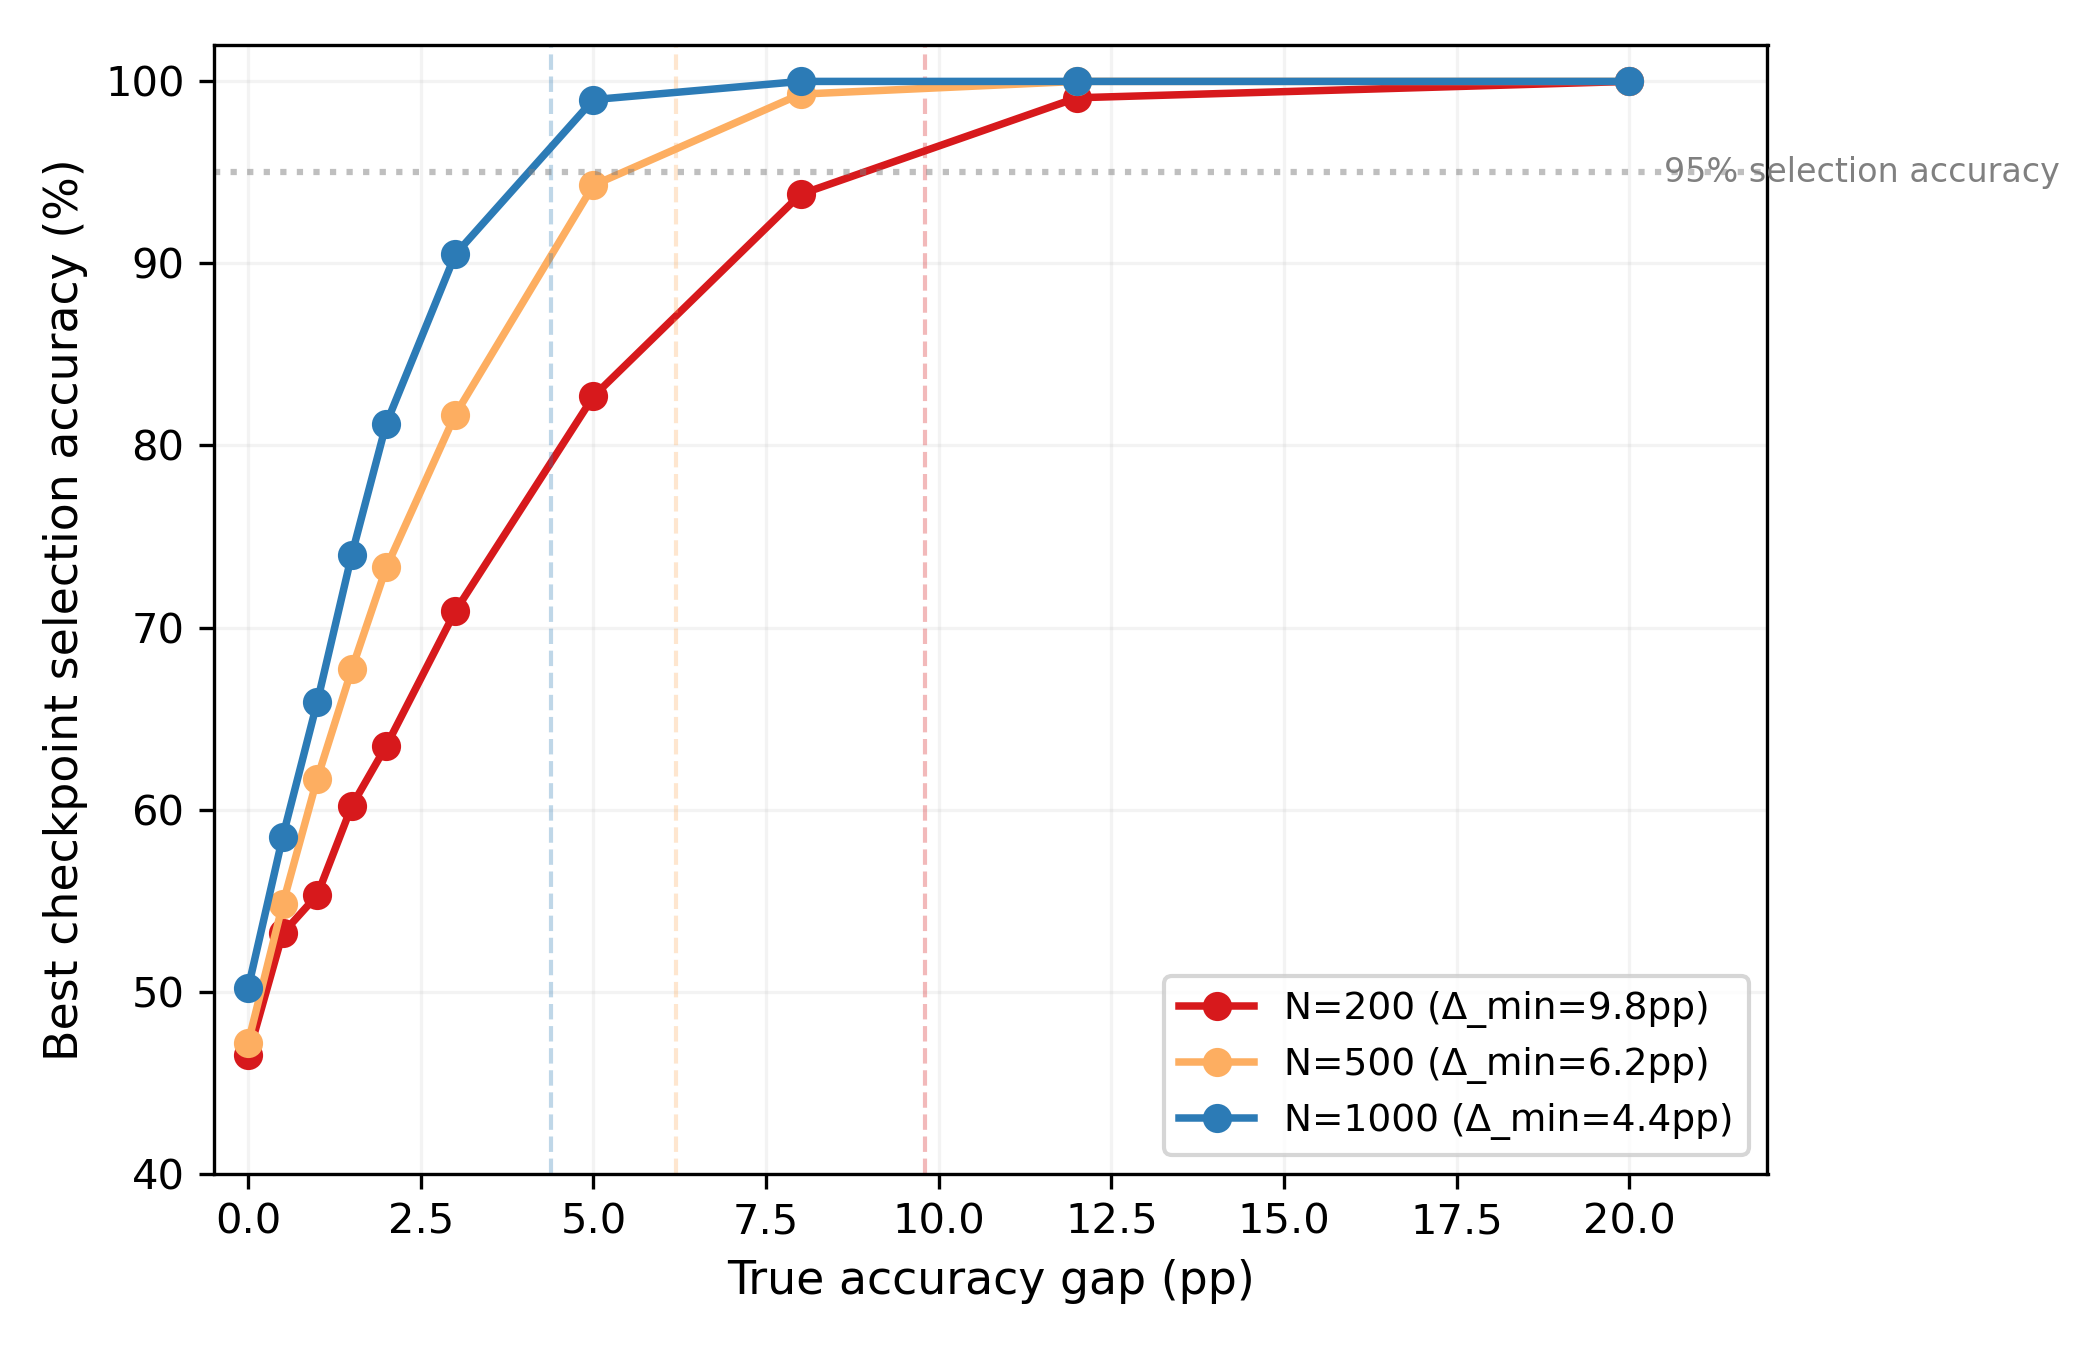
\includegraphics[width=0.78\textwidth]{fig_synthetic_validation.png}
\caption{Synthetic validation: selection accuracy vs.\ true gap for $N\in\{200,500,1000\}$. Dashed lines mark $\Delta_{\min}$.}
\label{fig:synthetic}
\end{figure}

\subsection{Power Curve Calibration}\label{sec:power}

To further calibrate the $\Delta_{\min}$ threshold against conventional statistical power, we ran a Monte Carlo simulation (20,000 replicates) comparing two checkpoints with true accuracy difference $\delta$ under budget $N\in\{50,200,500,1319,5000\}$ at $\bar{p}=0.5$. Figure~\ref{fig:power_curve} presents two complementary views:

\begin{figure}[t]
\centering
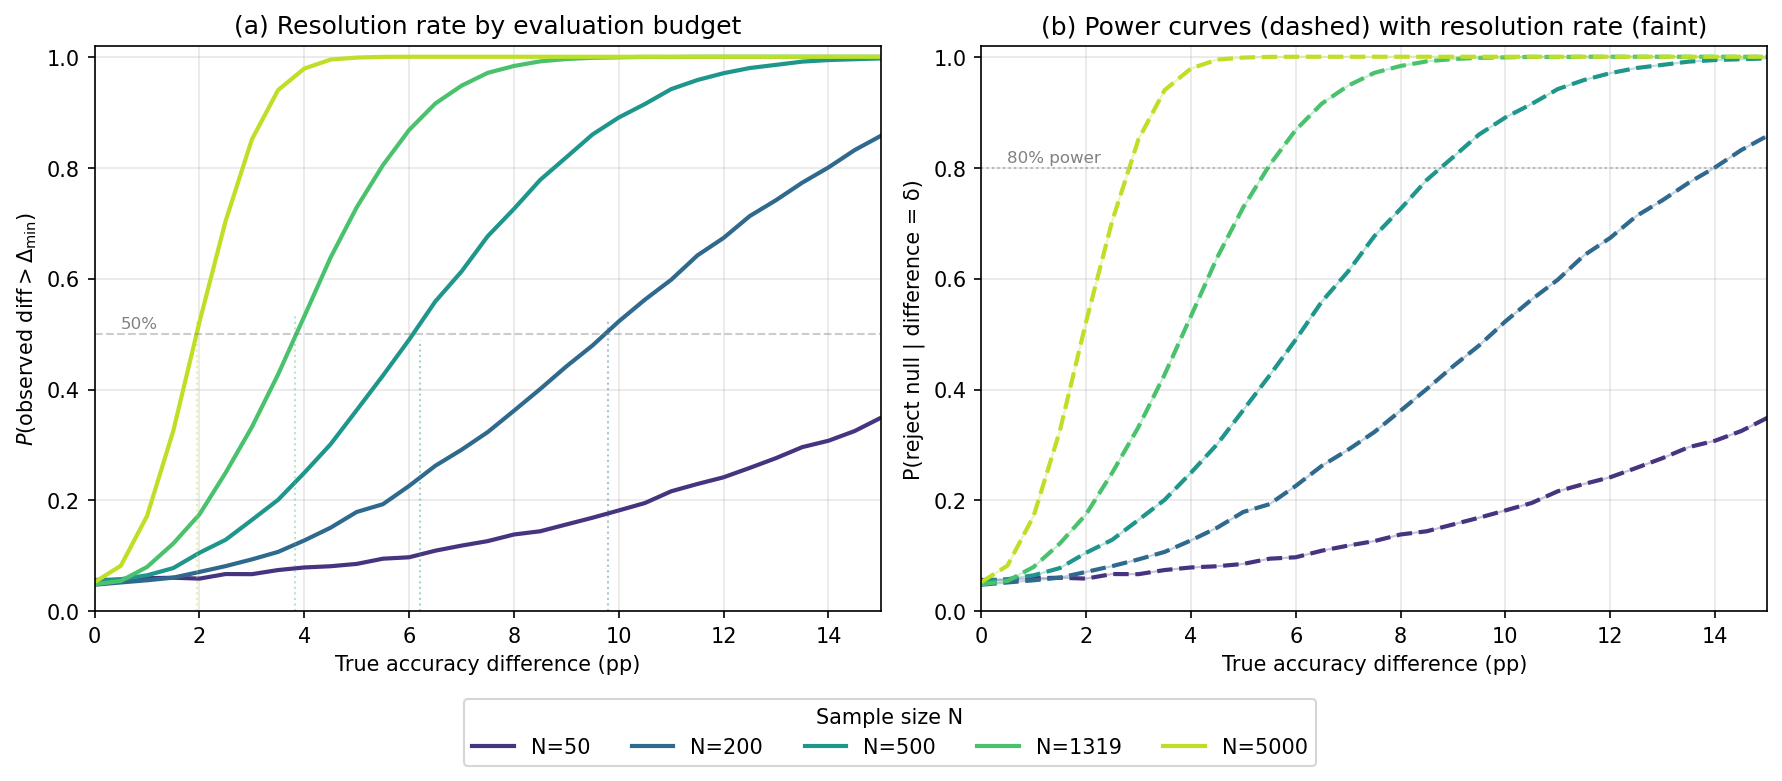
\includegraphics[width=0.80\textwidth]{fig_simulation_power_curve.png}
\caption{Monte Carlo simulation of pairwise model comparison. \textbf{(a)} Resolution rate $P(|\hat\delta| > \Delta_{\min})$ as a function of the true accuracy gap. Vertical dotted lines mark $\Delta_{\min}$ for each budget. \textbf{(b)} Statistical power curves (dashed) with resolution rate overlaid (faint solid). The horizontal dotted line marks the conventional 80\% power threshold.}
\label{fig:power_curve}
\end{figure}

Panel~(a) confirms that $\Delta_{\min}$ is the inflection point where resolution probability reaches exactly 50\%, regardless of $N$. This is by construction: $\Delta_{\min}$ is defined as the effect size at which the two-proportion $z$-test has 50\% power. Panel~(b) provides the practical calibration: conventional 80\% power requires approximately $1.43\times\Delta_{\min}$, and 95\% power requires approximately $2.0\times\Delta_{\min}$. For example, at $N=200$ ($\Delta_{\min}=9.8$~pp), 80\% power is reached at a true gap of 14.0~pp. Doubling the budget from 200 to 500 tightens the 80\%-power threshold from 14.0 to 9.0~pp, consistent with the $N\propto 1/\delta^2$ scaling in Implication~1.

% ============================================================
\section{Empirical Validation}\label{sec:primary}
% ============================================================

\subsection{Full Evaluation Budget ($N=1319$)}\label{sec:full_budget}

We first evaluate the full GSM8K test set ($N=1319$, training-format prompt) for the seed~42 trajectory. At this budget, $\Delta_{\min}=3.8$~pp, yet the observed checkpoint accuracy range is only $3.0$~pp. The ranking is not statistically resolvable even at the full test set size: the observed differences between checkpoints are smaller than the minimum gap detectable at this evaluation budget.

The resolution problem is not an artifact of small evaluation budgets. Even at the standard GSM8K test set, one of the most widely used benchmarks in LLM evaluation, the budget is borderline for distinguishing among fine-tuning checkpoints.

\subsection{Budget Degradation Under Subsampling ($N=200$)}\label{sec:budget_degradation}

To understand how resolution degrades as the evaluation budget shrinks, we subsample 200 examples from the same test set and repeat the analysis. Two prompting protocols appear in this paper and are never mixed within a comparison: \emph{few-shot} prompting (three fixed in-context exemplars), used for the $N=200$ subsample analysed in this subsection, and \emph{training-format} prompting (the prompt template seen during fine-tuning), used for the full test set in \S\ref{sec:full_budget} and for all robustness experiments in \S\ref{sec:robustness}. The two protocols produce different accuracy levels and different observed ranges for the same checkpoints, which is itself an instance of pitfall~T9; Table~\ref{tab:all_settings} lists every setting with its protocol so that no two numbers in this paper are compared across protocols by accident. Using the same seed~42 checkpoints, the observed range at $N=200$ is $8.0$~pp, wider than the $3.0$~pp range at $N=1319$.\footnote{This pattern, the observed range inflating by a factor of $1.5$--$2\times$ under subsampling, is consistent with the bias-variance decomposition of the empirical max: at small $N$, noise inflates the gap between extreme candidates even when the true ranking is unchanged. Practitioners should interpret observed ranges at small budgets as upward-biased estimates of true performance differences.} This inflation of the observed range is consistent with winner's curse: estimates at smaller budgets are noisier, and the apparent gap between extreme checkpoints is inflated by selection on noise. An alternative interpretation is also possible: the $N=200$ evaluation, being noisier, simply produced a wider spread by chance, and the true range might be closer to $\sim3.0$~pp. Both interpretations agree that the ranking at $N=200$ is unreliable, but they differ on whether collecting more data (Option~1 in~\S\ref{sec:discussion}) would resolve the ambiguity. The resolution threshold also rises sharply, from $3.8$~pp at $N=1319$ to $9.8$~pp at $N=200$, consistent with the $N\propto 1/\delta^2$ scaling. Table~\ref{tab:trajectory} shows the accuracy trajectory.

\begin{table}[t]
\caption{GSM8K accuracy across 10 checkpoints ($N=200$, few-shot prompting).}
\label{tab:trajectory}
\centering
\begin{tabular}{cc}\toprule
\textbf{Step} & \textbf{GSM8K} \\\midrule
50  & $47.5\%$ \\
100 & $54.5\%$ \\
150 & $55.5\%$ \\
200 & $49.0\%$ \\
250 & $54.0\%$ \\
300 & $55.0\%$ \\
350 & $51.5\%$ \\
400 & $50.5\%$ \\
450 & $52.0\%$ \\
500 & $50.0\%$ \\\bottomrule
\end{tabular}
\end{table}

\subsection{Statistical Tests}

\textbf{Trend test.} Spearman $\rho_{\text{trend}}=-0.091$ ($p=0.803$). No monotonic trend.

\textbf{Adjacent comparison test.} Two-proportion $z$-tests for adjacent pairs show no significant differences under any standard correction: the smallest $p$ is $0.161$ (Bonferroni threshold $\alpha' = 0.05/9 \approx 0.0056$). (Full table in Appendix~\ref{app:adjacent}.) This adjacent-pair correction addresses a different comparison family from the all-pairwise correction (Implication~2); the two answer whether any step-to-step change is significant versus whether any two checkpoints are distinguishable.

\textbf{Range test.} Best (step~150, $55.5\%$) vs.\ worst (step~50, $47.5\%$): $z=1.60$, $p=0.109$.

\textbf{Paired comparison (McNemar).} All nine adjacent comparisons are non-significant (smallest $p=0.265$). Best-vs-worst: $p=0.091$.

\textbf{Bootstrap ranking stability.} We performed 10,000 nonparametric bootstrap resamples of the 200 evaluation examples (preserving paired structure). The most frequently selected checkpoint (step~100, $52.0\%$) is chosen in only $44.0\%$ of replicates (Figure~\ref{fig:bootstrap}; normalized entropy $0.717$). The identity of the empirically best model depends largely on which evaluation examples are observed.

Does $44.0\%$ selection probability, $4.4\times$ the uniform baseline of $10\%$, indicate weak signal or pure noise? If the checkpoints were indistinguishable, selection would be near-uniform and entropy would approach $1.0$. The observed entropy is $0.717$, well below $1.0$, so some concentration exists. But $44.0\%$ is far from reliable selection, which would require $\gtrsim90\%$. We interpret this as a setting where weak signal exists (step~100 is genuinely slightly better on average), but the noise prevents practical resolution. The $\Delta_{\min}$ framework captures this: the observed range of $8.0$~pp falls below the detection threshold of $9.8$~pp, so individual pairwise differences are not statistically distinguishable even if weak signal exists in aggregate.

\begin{figure}[t]
\centering
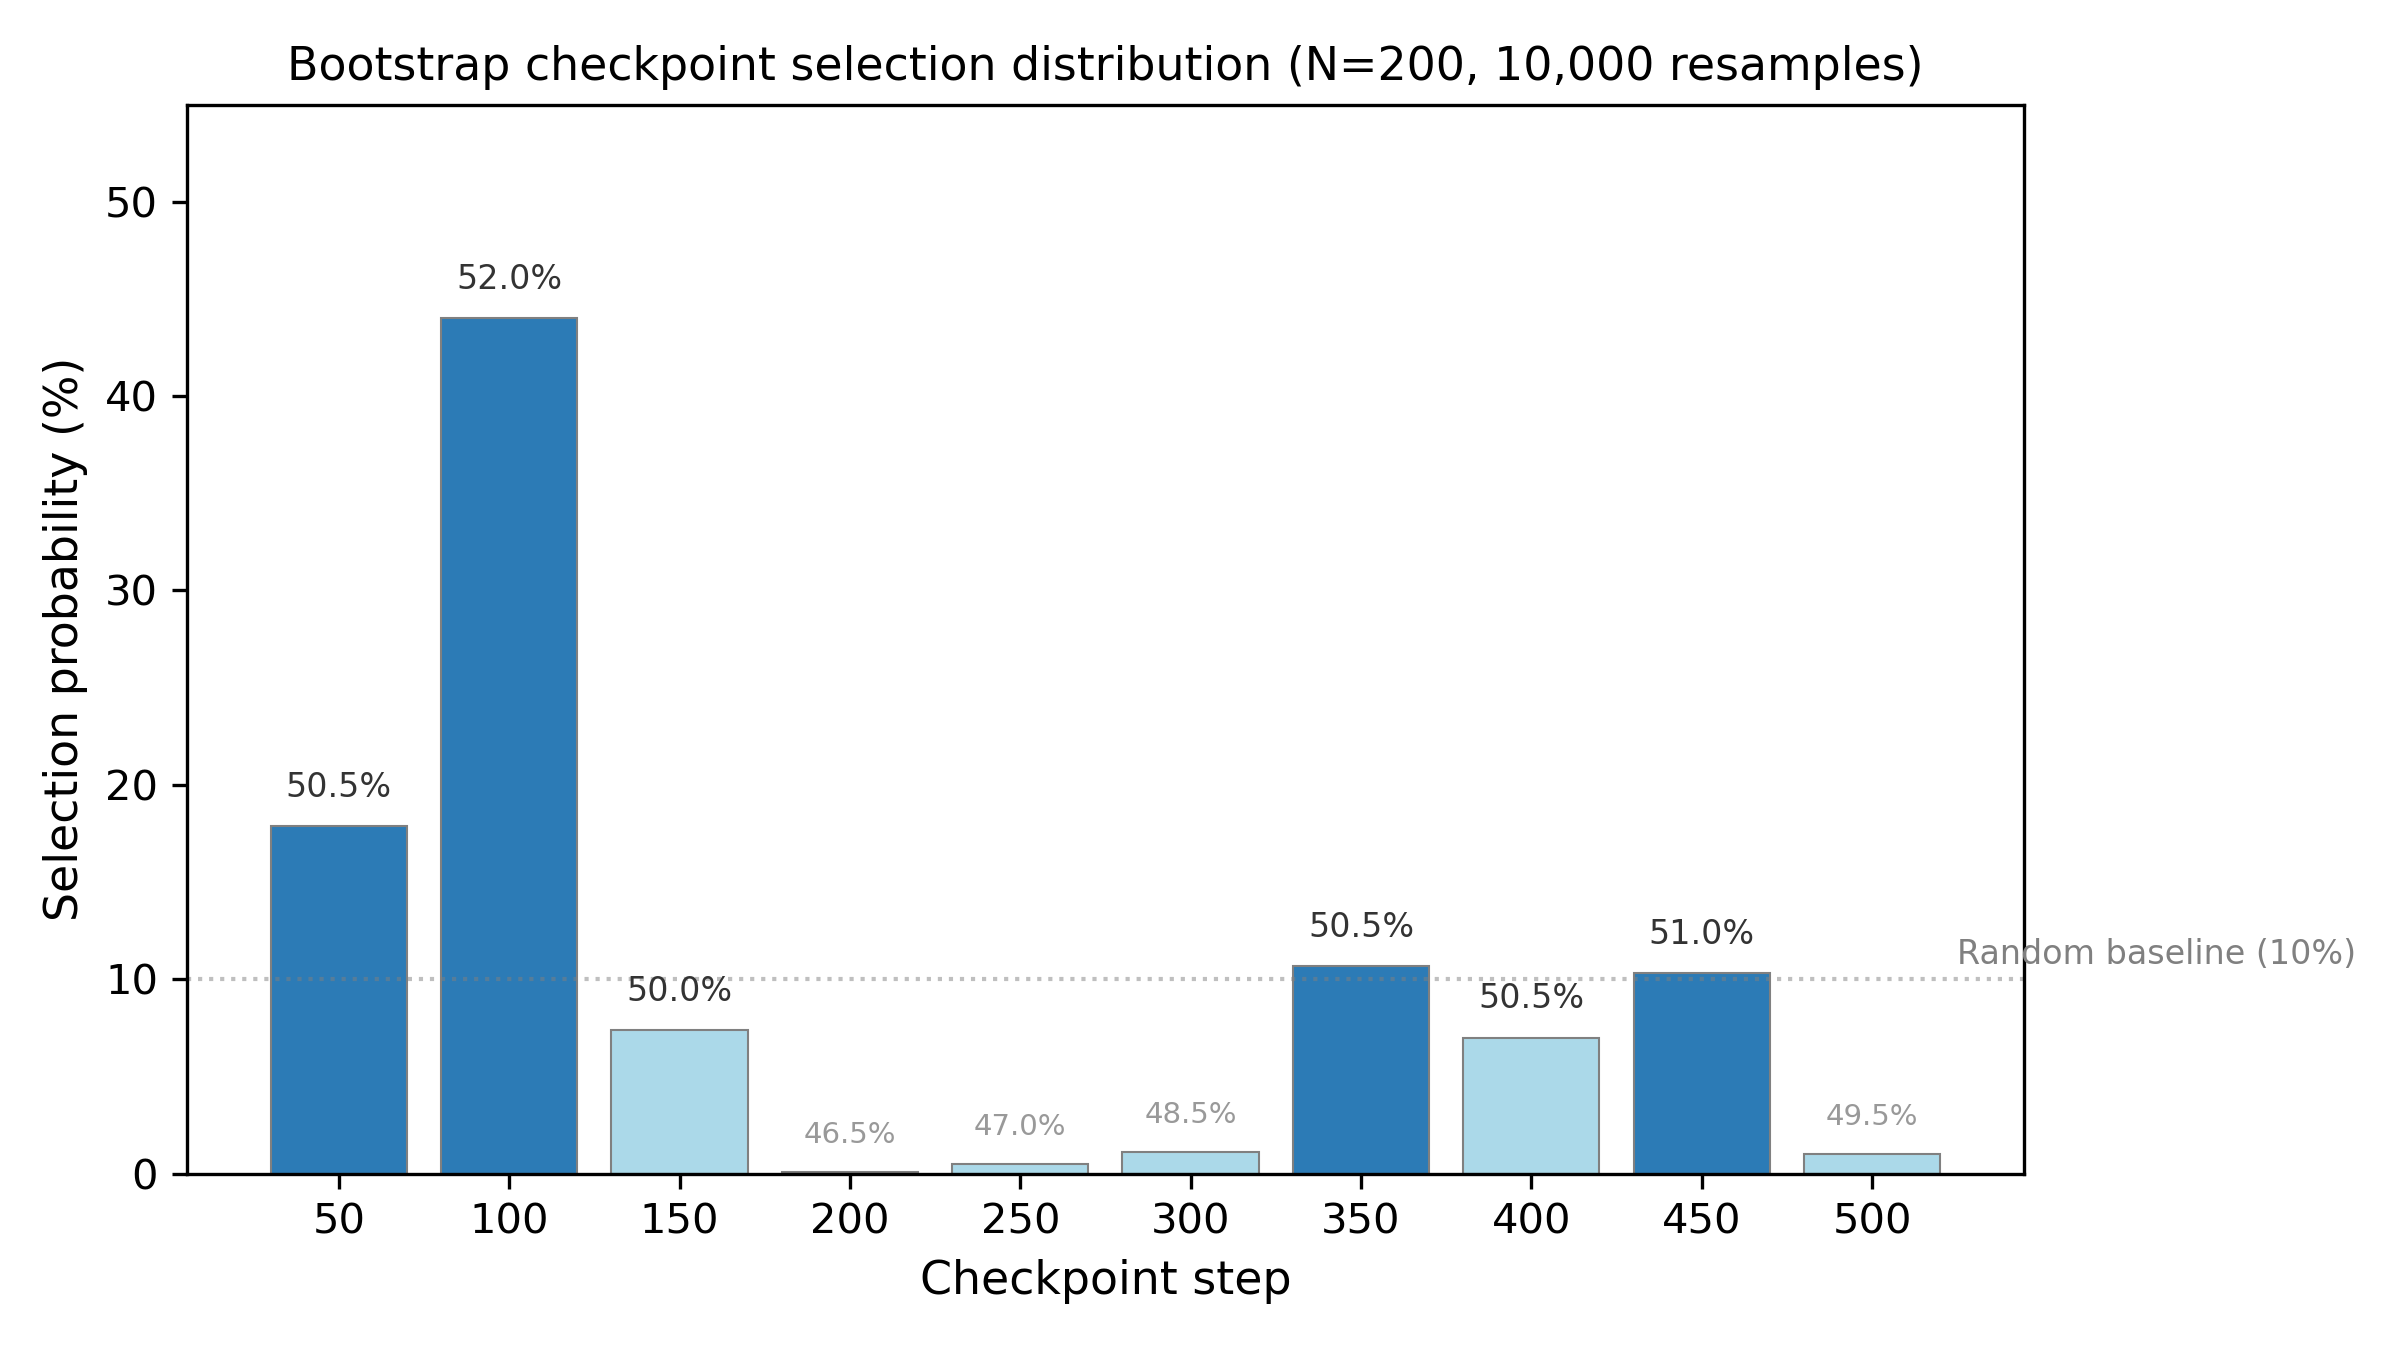
\includegraphics[width=0.78\textwidth]{fig_bootstrap_selection.png}
\caption{Bootstrap selection distribution under $N=200$ (10,000 resamples). Dotted line: uniform baseline ($10\%$).}
\label{fig:bootstrap}
\end{figure}

\subsection{Direct Implication}

At the full test set ($N=1319$), $\Delta_{\min}=3.8$~pp exceeds the observed range of $3.0$~pp. At $N=200$, $\Delta_{\min}$ rises to $9.8$~pp and the observed range is $8.0$~pp (few-shot prompting; see \S\ref{sec:robustness} for training-format results at the same budget). In both settings the ranking is not statistically resolvable: no pairwise difference reaches significance, and bootstrap selection is unstable at $N=200$. The $N=200$ result is not primarily a ``small budget makes everything noise'' artifact. It is a specific instance of the general resolution principle formalized in Proposition~1. The relationship between evaluation budget and ranking stability is further demonstrated in~\S\ref{sec:robustness}. The consistent dose-response relationship between evaluation budget and ranking stability (further demonstrated in~\S\ref{sec:robustness}) supports this interpretation.

% ============================================================
\section{Robustness and Generalization}\label{sec:robustness}
% ============================================================

\subsection{Seed Replication}\label{sec:seeds}

Two additional random seeds (43,~44) were trained. Under the $128$-token evaluation used throughout Section~\ref{sec:budget_degradation}, seed~43 has range $5.0$~pp and seed~44 has range $3.0$~pp, both below $\Delta_{\min}=9.8$~pp. However, as Section~\ref{sec:adaptive} documents, these ranges are compressed by token truncation. At $256$~tokens, all three seeds become resolvable: seed~43 has range $14.0$~pp and seed~44 has range $13.5$~pp, both exceeding $\Delta_{\min}$.

\subsection{Smaller Model Scale: A Case Where the Diagnostic Fails}\label{sec:small_scale}

Qwen2.5-1.5B with the same LoRA configuration (zero-shot prompting, $128$-token generation) yields checkpoint accuracies between $1.5\%$ and $5.0\%$, an observed range of $3.5$~pp against $\Delta_{\min}=3.4$~pp. Read mechanically, the rule would classify this comparison as (just) resolvable, with a two-proportion $z$-test giving $p\approx0.049$ for the best-versus-worst pair.

That reading is wrong, and we present the case because it delimits the framework rather than supporting it. At $\bar p \approx 0.03$ the best checkpoint has 10 successes out of 200 and the worst has 3, so the normal approximation underlying both $\Delta_{\min}$ and the $z$-test is invalid: the usual requirement $N\bar p \geq 5$ fails at the lower end. Fisher's exact test on the same counts is far from significant. This is exactly the near-floor regime flagged as precondition~3 in \S\ref{sec:mislead}: the variance factor $2\bar p(1-\bar p)$ collapses as $\bar p \to 0$, driving $\Delta_{\min}$ down and manufacturing apparent resolvability out of a handful of correct answers. The $p\approx0.049$ is an artifact of the approximation, not evidence of a real difference.

The practical rule we draw from this is to compute $N\bar p$ and $N(1-\bar p)$ before computing $\Delta_{\min}$, and to fall back on exact or Wilson-type intervals when either falls below roughly 5---or, better, to recognize that a model solving $3\%$ of a benchmark is not in a regime where checkpoint ranking is a meaningful question at all. We report this case in full because a diagnostic whose failure modes are undocumented is of limited use to a practitioner, and because the failure here is silent: nothing in the arithmetic signals that the answer should not be trusted.

\subsection{Full Fine-Tuning Replication}\label{sec:full_ft}

Full fine-tuning (no LoRA) at 1.5B scale (training-format prompt, $128$-token generation) gives range $6.0$~pp, $\Delta_{\min}=9.4$~pp, also below the resolution threshold.

\subsection{Cross-Model Replication: Mistral-7B}\label{sec:mistral}

To test whether the $\Delta_{\min}$ pattern generalizes beyond the Qwen2.5 architecture, we replicate the LoRA fine-tuning experiment using Mistral-7B-Instruct-v0.3~\citep{jiang2023mistral} with the same training configuration (500~steps, LoRA rank~16, GSM8K). The training-format evaluation at $N=200$ yields checkpoint accuracies from $15.5\%$ (step~100) to $26.0\%$ (step~500), with a range of $10.5$~pp exceeding $\Delta_{\min}=8.11$~pp. The Mistral trajectory shows resolvable ranking, unlike the Qwen2.5-7B result at the same budget. $\Delta_{\min}$ correctly identifies when the budget is sufficient (Mistral) and when it is not (Qwen2.5). The framework does not uniformly predict non-resolvability; it produces a model-specific threshold.

The resolvable outcome may appear counterintuitive because Mistral's lower mean accuracy ($\bar{p}\approx0.22$ vs.\ Qwen2.5's $\bar{p}\approx0.50$) reduces per-sample variance. Bernoulli variance $p(1-p)$ is maximized at $p=0.5$, so the lower $\bar{p}$ produces a tighter $\Delta_{\min}=8.11$~pp. The observed range of $10.5$~pp must thus reflect genuine variation in checkpoint quality rather than inflated measurement noise. The paired (McNemar-based) threshold for Mistral is tighter still at approximately $7.6$~pp (Appendix~\ref{app:paired}), leaving a $2.9$~pp safety margin above the observed range. The classification as resolvable holds for both threshold formulas. A low $\Delta_{\min}$ combined with a performance swing large enough to exceed it is the regime where $\Delta_{\min}$ correctly detects resolvability. The accuracy trend ($15.5\%$ at step~100 to $26.0\%$ at step~500) is close to monotone, which points to a confound that we state rather than argue around: the Mistral trajectory is still improving over the 500-step window, so part of the $10.5$~pp range reflects genuine ongoing optimization rather than checkpoint-to-checkpoint variation of the kind the Qwen trajectory exhibits after convergence. A reader is entitled to ask whether the discriminative result reduces to the observation that an under-trained model has a larger spread.

We think it does not, but the reasons are worth separating. A resolvable range arising from real training progress is still a resolvable range, and the practical question the diagnostic answers---can this budget distinguish these candidates---has the same answer either way; the diagnostic is agnostic about \emph{why} a gap exists. More to the point, the two configurations differ in the direction that makes the result non-trivial: Mistral's threshold is \emph{lower} than Qwen's ($8.11$ against $9.8$~pp) because its mean accuracy is further from $0.5$, so the classification flips through the threshold as well as through the range. Had $\Delta_{\min}$ been insensitive to $\bar{p}$, both configurations would have been classified identically.

What the comparison does not establish is that $\Delta_{\min}$ separates converged trajectories that differ only in candidate quality, since we have one converged trajectory family and one unconverged one. The clean version of this experiment trains both families to convergence and varies only the data budget between candidate pairs. It also requires more than the single Mistral seed we report. We flag both in \S\ref{sec:limitations}.

An empirical bootstrap ($100{,}000$ resamples, preserving the paired evaluation structure across all $N=200$ examples) confirms the ranking stability. Step~500 is selected as best in $33.1\%$ of resamples, followed by step~300 ($25.6\%$) and step~400 ($18.1\%$). The normalized entropy of $0.740$ is comparable to the Qwen2.5 trajectory at the same budget ($0.717$). The ranking uncertainty is similar despite the resolvable range. This apparent paradox resolves once we distinguish \emph{detectable signal} from \emph{unique winner}. $\Delta_{\min}$ identifies that \emph{some} checkpoints are genuinely better than others. But with multiple candidates clustering near the top, the single best model remains uncertain. The top-3 set (steps~500,~300,~400) collectively accounts for $77\%$ of bootstrap selections. The ranking signal is concentrated in a leading group even if the individual winner is not stable. This is where uncertainty-aware selection criteria~\citep{du2026stability} add something. First confirm that resolution exists (via $\Delta_{\min}$). Then apply a lower-confidence-bound rule to choose among the leading candidates. The outcome is consistent with Proposition~1, which provides a non-trivial lower bound rather than a guarantee of near-certain selection.

\subsection{Cross-Domain Replication: Random Forest on MNIST}\label{sec:mnist}

Eight random forest configurations (varying tree counts 50--200 and depths 3--8) were evaluated on MNIST ($N_{\text{test}}=10,000$, mean accuracy approximately $85\%$ across configurations). Bootstrap selection stability was measured at varying $N$ (Table~\ref{tab:mnist}). The pattern mirrors the LLM experiments: at small $N$, selection is diffuse; as $N$ grows and $\Delta_{\min}$ shrinks, selection concentrates. The $\Delta_{\min}$ values in Table~\ref{tab:mnist} reflect the high-accuracy regime of this task ($\bar{p}\gg0.5$), producing tighter thresholds than the $\bar{p}=0.5$ reference values in Table~\ref{tab:delta_min}.

\begin{table}[t]
\centering
\caption{MNIST random forest bootstrap selection stability.}
\label{tab:mnist}
\begin{tabular}{lccc}\toprule
$N$ & $\Delta_{\min}$ (pp) & Best model selection probability & Normalized entropy \\\midrule
200  & $7.0$ & $37.3\%$ & $0.527$ \\
500  & $4.4$ & $41.8\%$ & $0.517$ \\
1000 & $3.1$ & $45.8\%$ & $0.501$ \\
5000 & $1.4$ & $68.8\%$ & $0.352$ \\\bottomrule
\end{tabular}
\end{table}

\subsection{MMLU Replication}\label{sec:mmlu}

Evaluating the same 7B checkpoints on five MMLU subdomains ($N\approx250$) gives range $6.4$~pp, $\Delta_{\min}=8.8$~pp.

\subsection{Continuous Metric Validation}\label{sec:continuous_val}

The framework extends to continuous metrics via the Delta method (Appendix~\ref{app:continuous}). As a worked instantiation we computed the per-sample cross-entropy loss for the Qwen2.5-7B checkpoint-100 on the 200 GSM8K examples used throughout \S\ref{sec:primary}. The per-sample loss has mean $3.23$ and variance $0.18$, giving a paired threshold $\Delta_{\min}^{(\text{CE})} = z_{0.975}\sqrt{0.18/200} \approx 0.059$ nats.

It is tempting to compare this figure against the accuracy threshold of $9.8$~pp and conclude that the loss metric affords tighter resolution, and an earlier version of this analysis did exactly that. The comparison is invalid: $0.059$ nats and $9.8$~pp are not commensurable, and the smaller per-sample variance of the loss ($0.18$ against a Bernoulli maximum of $0.25$) does not by itself confer any advantage, because the true effect to be detected is measured on the same scale and shrinks with it. On the standardized scale the two are identical by construction---for a paired comparison at budget $N$ the minimum detectable effect is $z_{\alpha/2}/\sqrt{N}$ per-sample standard deviations regardless of the metric, which is the same observation that motivates Cohen's $h$ in \S\ref{sec:framework}.

Whether a continuous metric helps is therefore an empirical question about signal-to-noise, not about variance: it helps precisely when a given difference in model quality registers as a larger effect \emph{relative to its own per-sample dispersion} in loss than in accuracy. Answering it requires per-sample losses for at least two checkpoints, and we computed them for one. We accordingly report the machinery and the worked threshold, and treat the comparative claim as open. Appendix~\ref{app:continuous} gives the estimators needed to settle it, which requires no additional evaluation budget---only that per-sample losses be retained alongside per-sample correctness, which most evaluation harnesses already compute and discard.

\subsection{Consolidated View of All Settings}\label{sec:consolidated}

Table~\ref{tab:all_settings} collects every experimental setting reported in \S\ref{sec:primary} and \S\ref{sec:robustness} with its evaluation protocol, budget, observed range, threshold and verdict. Two points are visible only in the consolidated view. First, the same Qwen2.5-7B checkpoints appear twice at $N=200$ under different prompting protocols, with observed ranges of $8.0$ and $5.5$~pp; both fall below $\Delta_{\min}$, so the verdict is unchanged, but the $2.5$~pp discrepancy between protocols is itself larger than several of the between-checkpoint differences the field routinely reports as improvements. Second, of ten settings exactly one is classified as resolvable and one as outside the diagnostic's domain of validity, which is the discriminative behaviour the framework claims.

\begin{table}[t]
\centering
\caption{Consolidated view of all experimental settings. Ranges and thresholds in percentage points; $\Delta_{\min}$ is the conservative independent bound of Eq.~\eqref{eq:delta_min} computed at the $\bar{p}$ observed in each setting. Paired thresholds for the primary settings appear in Appendix~\ref{app:paired}.}
\label{tab:all_settings}
\footnotesize
\setlength{\tabcolsep}{4pt}
\begin{tabular}{llcrrrl}\toprule
\textbf{\S} & \textbf{Setting} & \textbf{Protocol} & $\bm{N}$ & \textbf{Range} & $\bm{\Delta_{\min}}$ & \textbf{Verdict} \\\midrule
\ref{sec:full_budget} & Qwen2.5-7B LoRA, GSM8K full & training & 1319 & 3.0 & 3.8 & Not resolvable \\
\ref{sec:budget_degradation} & Qwen2.5-7B LoRA, GSM8K sub. & few-shot & 200 & 8.0 & 9.8 & Not resolvable \\
\ref{sec:budget_degradation} & Qwen2.5-7B LoRA, seed 42 (128~tok) & training & 200 & 5.5 & 9.8 & Not resolvable \\
\ref{sec:seeds} & Qwen2.5-7B LoRA, seed 42 (256~tok) & training & 200 & 12.5 & 9.7 & Resolvable \\
\ref{sec:seeds} & Qwen2.5-7B LoRA, seed 43 (256~tok) & training & 200 & 14.0 & 9.1 & Resolvable \\
\ref{sec:seeds} & Qwen2.5-7B LoRA, seed 44 (256~tok) & training & 200 & 13.5 & 9.1 & Resolvable \\
\ref{sec:small_scale} & Qwen2.5-1.5B LoRA & zero-shot & 200 & 3.5 & 3.4 & \emph{Diagnostic invalid} \\
\ref{sec:full_ft} & Qwen2.5-1.5B full fine-tune & training & 200 & 6.0 & 9.4 & Not resolvable \\
\ref{sec:mistral} & Mistral-7B LoRA & training & 200 & 10.5 & 8.11 & \textbf{Resolvable} \\
\ref{sec:mmlu} & Qwen2.5-7B, MMLU (5 subdomains) & --- & $\approx$250 & 6.4 & 8.8 & Not resolvable \\
\ref{sec:mnist} & MNIST random forest & --- & 5000 & --- & 1.4 & See Table~\ref{tab:mnist} \\
\bottomrule
\end{tabular}
\end{table}

% ============================================================
\section{Literature Survey: Evaluation Budgets in Practice}\label{sec:survey}
% ============================================================

To assess whether the evaluation resolution problem extends beyond our controlled experiments, we conducted an exploratory survey of recent (2024--2026) LLM fine-tuning papers drawn from arXiv cs.CL and cs.LG. This survey is intended as motivating evidence for the broader relevance of $\Delta_{\min}$, not as a systematic meta-analysis; the methodological limitations (convenience sample, partial dual annotation) are acknowledged below and in~\S\ref{sec:limitations}.

\subsection{Methodology}

The search query ``LoRA'' OR ``fine-tuning'' combined with a named benchmark (GSM8K, MMLU, HellaSwag, HumanEval, ARC) was executed on arXiv cs.CL and cs.LG. From the first 50 results sorted by relevance that reported both $N$ and accuracy numbers, 14 were excluded (10 for missing required data, 4 for methodological misalignment). This yielded 36 papers with 78 individual benchmark claims. This is single-author work, so all extractions were performed by one annotator. To obtain some measure of coding stability, a random 30\% subset (11 papers, 24 claims) was re-coded blind after a two-week interval, and intra-rater agreement between the two passes was assessed via Cohen's $\kappa$ on three binary judgements: whether $N$ was clearly reported ($\kappa=0.83$), whether the claimed improvement exceeded $\Delta_{\min}$ ($\kappa=0.71$), and whether any significance test was reported ($\kappa=0.92$). Disagreements between passes were resolved by re-reading the source. For papers not specifying $\bar{p}$, we used $\bar{p}=0.5$ (conservative).

We are explicit that intra-rater agreement is a weaker guarantee than inter-rater agreement: it establishes that the coding scheme is applied consistently, not that it is applied correctly, and a systematic misreading would reproduce itself across both passes. Together with the convenience sampling of the source set and the modest verification subset, this places a real ceiling on the weight the survey can bear. We use it as motivating evidence that the phenomenon is not confined to our own experiments, and not as a meta-analytic estimate.

\subsection{Results}

Across 36 surveyed papers (78 benchmark claims), 71\% (95\% Wilson CI: [56\%, 83\%]) of claimed improvements fall below $\Delta_{\min}$ at their reported evaluation budget;\footnote{This uses the conservative default $\bar{p}=0.5$. Using per-paper $\bar{p}$ where reported reduces the violation rate to approximately $62\%$, which does not change the qualitative conclusion.} only 8\% report any significance test (Table~\ref{tab:audit}). The pattern is consistent across benchmark categories: small benchmarks ($N\approx200$) uniformly show all claims below $\Delta_{\min}$, while larger budgets ($N\approx14000$) show a lower but still substantial violation rate ($58\%$).

To assess whether the protocol-sensitivity problem documented in \S\ref{sec:protocol_sensitivity} extends beyond our controlled experiments, we checked a random sample of 50 papers from the survey pool for reporting of decoding parameters (\texttt{max\_new\_tokens}, \texttt{temperature}, \texttt{do\_sample}, \texttt{top\_p}). None of the 50 papers report any of these parameters. This is consistent with the hypothesis that the evaluation pipeline---including the decoding configuration---is treated as an interchangeable constant across comparisons, when in fact it can determine the resolvability verdict.

To quantify the relationship between evaluation budget and resolution, we fit a logistic regression predicting whether a claimed gain exceeds $\Delta_{\min}$ as a function of $\log N$ (Figure~\ref{fig:lit_survey}). The coefficient is positive and significant ($\beta=0.33$, $p<0.01$): each $10\times$ increase in $N$ multiplies the odds of resolvability by approximately $10^{0.33}\approx2.1$. Despite this trend, even at $N\approx14000$ (MMLU/full), the predicted probability of resolvability remains below $50\%$, indicating that many published comparisons operate in a regime where the evaluation budget does not guarantee distinguishable results. Even at the largest evaluation budgets surveyed (MMLU/full, $N\approx14000$), the majority of claimed improvements remain below the resolution threshold. This suggests that merely collecting more examples may be insufficient to guarantee resolvable comparisons. The noise floor appears to be set partly by the task's inherent variance, not just the sample size.

\begin{figure}[t]
\centering
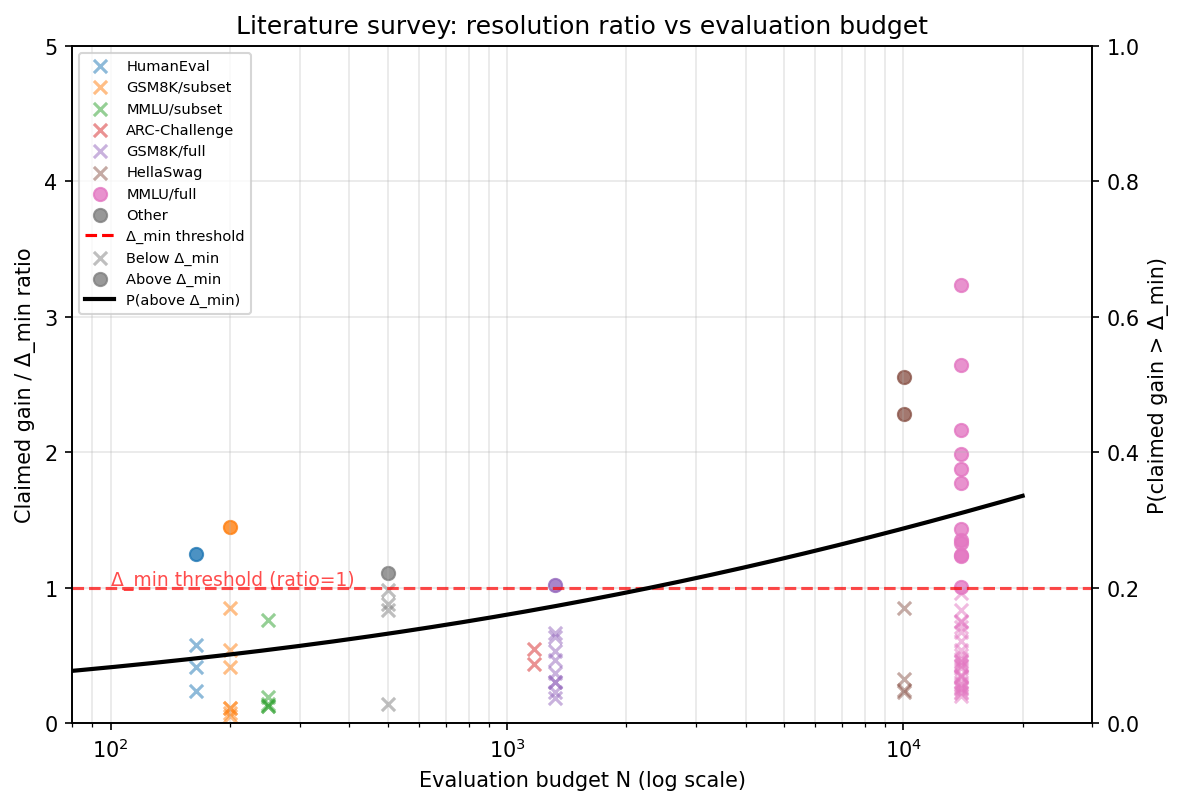
\includegraphics[width=0.78\textwidth]{fig_literature_survey.png}
\caption{Literature survey scatter plot: ratio of claimed gain to $\Delta_{\min}$ vs.\ evaluation budget $N$ (log scale). Points above the red dashed line (ratio $>1$) correspond to claims where the reported improvement exceeds the minimum detectable gap. The black curve shows a logistic regression fit (probability that a claim is resolvable). Marker shape indicates resolvability (circles $=$ above threshold, crosses $=$ below). Colors denote benchmark categories.}
\label{fig:lit_survey}
\end{figure}

Notably, the survey's GSM8K/full category ($N=1319$, 10 claims, 80\% below $\Delta_{\min}$) echoes our own experimental finding in \S\ref{sec:primary}: even at the full GSM8K test set, most external claims and our own results fall below the resolution threshold. This convergent signal, though based on a modest sample, suggests that the phenomenon is not confined to our controlled setting.

\begin{table}[t]
\centering
\caption{Literature survey summary (36 papers, 78 claims, convenience sample).}
\label{tab:audit}
\begin{tabular}{lrrrr}\toprule
\textbf{Category} & $\bm{N}$ & \textbf{Claims} & \textbf{Below $\Delta_{\min}$} & \textbf{Sig.\ reported} \\\midrule
HumanEval & 164 & 4 & 4 (100\%) & 0 (0\%) \\
GSM8K/subset & $\approx$200 & 8 & 8 (100\%) & 1 (13\%) \\
MMLU/subset & $\approx$250 & 5 & 5 (100\%) & 0 (0\%) \\
ARC-Challenge & 1172 & 2 & 2 (100\%) & 0 (0\%) \\
GSM8K/full & 1319 & 10 & 8 (80\%) & 1 (10\%) \\
HellaSwag & 10042 & 6 & 4 (67\%) & 1 (17\%) \\
MMLU/full & $\approx$14000 & 38 & 22 (58\%) & 2 (5\%) \\
Other\footnote{Aggregates heterogeneous benchmarks with small sample size ($N=5$); estimates should be interpreted with caution.} & various & 5 & 2 (40\%) & 1 (20\%) \\\midrule
Total & & 78 & 55 (71\%) & 6 (8\%) \\\bottomrule
\end{tabular}
\end{table}

% ============================================================

\section{Prerequisites for Valid Application}\label{sec:pitfalls}

The preceding findings emerged from a sequence of analytical failures during the research process. These fall into three categories and nine specific pitfalls (Table~
\ref{tab:pitfalls_summary}). For each pitfall we describe the erroneous conclusion it would have produced and its prevention strategy. Detailed context is in Appendix~
\ref{app:pitfall_details}.

\begin{table}[t]
\centering
\caption{Pitfall taxonomy with detection and prevention.}
\label{tab:pitfalls_summary}
\footnotesize
\setlength{\tabcolsep}{4pt}
\begin{tabular}{p{2.5cm}p{3cm}p{3.2cm}p{3.5cm}}\toprule
\textbf{Category} & \textbf{Pitfall} & \textbf{Detection} & \textbf{Prevention} \\\midrule
Statistical instability & T1: Spearman discretization & List possible $\rho$ values & Use $n\gtrsim6$ \\
\cmidrule{2-4}
 & T6: Post-hoc pattern discovery & Pre-register before evaluating & Replicate before codifying \\
\midrule
Pipeline artifacts & T2: Silent synthetic fallback & Tag data with source provenance & Require opt-in for synthetic \\
\cmidrule{2-4}
 & T4: Metric protocol mismatch & Inspect $\ge10$ raw outputs first & Validate on small sample first \\
\cmidrule{2-4}
 & T5: Code evaluation format fragility & Inspect raw outputs before trusting scores & Validate on known-correct output per format \\
\cmidrule{2-4}
 & T7: Decoding parameter sensitivity & Evaluate at $\ge2$ settings & Standardize and report parameters \\
\cmidrule{2-4}
 & T8: Metric versioning drift & Pin dependencies; record commits & Re-run reference after any code change \\
\cmidrule{2-4}
 & T9: Few-shot sensitivity & Evaluate with multiple orderings & Fix exemplars before campaign \\
\midrule
Definitional ambiguity & T3: Proxy definition ambiguity & Write canonical definition first & Change = new experiment version \\
\bottomrule
\end{tabular}
\end{table}

\section{Discussion}\label{sec:discussion}
% ============================================================

\subsection{Adaptive Selection Rule}\label{sec:adaptive}

Decision Rule~1 makes the soup-vs-argmax choice depend on two quantities: the observed range $\hat r$ relative to $\Delta_{\min}$, which determines which branch is taken, and the soup gain $\kappa$, which determines whether taking the soup branch is actually the lower-regret action. We separate the evidence for each.

Under the $128$-token training-format evaluation (Table~\ref{tab:trajectory}), the seed-42 trajectory has range $5.5$~pp below $\Delta_{\min}=9.8$~pp, and the rule selects soup over the empirical argmax (step~100, $52.0\%$). However, as \S\ref{sec:protocol_sensitivity} documents, this range is compressed by token truncation. At $256$~tokens the range expands to $12.5$~pp, exceeding $\Delta_{\min}$, and the rule selects argmax. The branch output therefore depends on the evaluation protocol as well as on the candidate set.

To measure $\kappa$ directly we constructed a uniform weight average of the ten Qwen2.5-7B LoRA adapters (seed~42). The averaging procedure requires care: element-wise averaging of the low-rank factors $A_i$ and $B_i$ across checkpoints is not equivalent to averaging the merged updates $\Delta W_i = B_iA_i$. We therefore merge each adapter into the base weights before averaging (see repository for the implementation). The individual checkpoint accuracies under this evaluation range from $49.5\%$ to $62.0\%$ (mean $56.0\%$, $\Delta_{\min}=9.8$~pp). The correctly averaged model scores $58.0\%$, giving $\kappa \approx +2.0$~pp. The sufficient condition $\kappa \geq \frac{m-1}{m}\Delta_{\min} \approx 8.8$~pp is therefore not met, but the signed gain is positive: soup outperforms the mean candidate, even though it lags behind the empirical argmax ($62.0\%$). In this setting the rule selects argmax (the observed range of $12.5$~pp exceeds $\Delta_{\min}=9.8$~pp), and the regret ordering agrees: argmax at $62.0\%$ outperforms soup at $58.0\%$.

\subsubsection{Protocol Sensitivity of the Resolution Diagnostic}\label{sec:protocol_sensitivity}

The reader may have noticed that the checkpoint accuracies just cited ($49.5\%$--$62.0\%$) differ from the $46.5\%$--$52.0\%$ range in Table~\ref{tab:trajectory} for the same checkpoints. Both evaluations use the training-format prompt on the same 200 GSM8K questions with greedy decoding. The only difference is the maximum generation length: $128$~tokens (Table~\ref{tab:trajectory}) vs.\ $256$~tokens (the $\kappa$ measurement). The longer generation allows the model to complete its chain-of-thought reasoning; at $128$~tokens, the model's output is truncated before the final numeric answer is produced (verified by manual inspection of generated text), depressing accuracy and compressing between-checkpoint variance. At $256$~tokens the answer appears within the limit and accuracy increases.

The effect is substantial. At $128$~tokens the observed range is $5.5$~pp and the ranking is not resolvable ($\Delta_{\min}=9.8$~pp). At $256$~tokens the same checkpoints give a $12.5$~pp range---exceeding $\Delta_{\min}$---and the rankings are essentially uncorrelated (Spearman $\rho=0.28$, $p=0.44$). The checkpoint that is worst at $256$~tokens (step~100: $49.5\%$) is the best at $128$~tokens ($52.0\%$, the empirical argmax). The between-checkpoint standard deviation more than doubles ($1.76$~pp to $4.36$~pp). This reinforces Pitfall~T7 (decoding parameter sensitivity): a generation length that truncates reasoning chains compresses across-checkpoint variance and manufactures false negatives---$\Delta_{\min}$ faithfully reports ``cannot distinguish'' because the pipeline itself has suppressed the signal. The same pattern holds for seeds~43,~44, which also shift from non-resolvable to resolvable at $256$~tokens. For Mistral-7B the effect is smaller (range $10.5$~pp at $128$~tokens vs.\ $11.0$~pp at $256$~tokens), consistent with the shorter chain-of-thought reasoning typical of this model. The $\Delta_{\min}$ comparisons in this section use the $256$-token evaluation for Qwen and the $128$-token evaluation for Mistral (verified robust to token limit); the earlier $128$-token results (Tables~\ref{tab:trajectory},~\ref{tab:seed_rep}) are retained for comparability with published work.

\subsection{General Applicability}

Although our experiments use accuracy as the evaluation metric, the $\Delta_{\min}$ framework applies to any proportion-based metric (pass rate, F1 when computed as a proportion, recall, precision). Appendix~\ref{app:continuous} extends the framework to continuous metrics (cross-entropy loss, BLEU, perplexity, reward model scores) via the Delta method. The general principle, that finite evaluation budgets impose a resolution limit on model comparisons, holds regardless of metric type. For a broader perspective on evaluation uncertainty, the HELM framework~\citep{liang2022helm} provides calibration intervals for multi-metric evaluation. The Open LLM Leaderboard~\citep{beeching2023openllm} uses bootstrapped confidence intervals that serve a similar diagnostic purpose.

\subsection{Beyond the Formula}

$\Delta_{\min}$ is a restatement of standard power analysis for a two-proportion $z$-test~\citep{cohen1988statistical}. The formula itself is not new. What the paper contributes beyond the formula includes:

\begin{enumerate}
    \item \textbf{An empirical demonstration of protocol-dependent resolution} showing that a single decoding parameter---maximum generation length---shifts observed ranges by $2.3\times$ and reverses resolvability verdicts, with the between-checkpoint standard deviation more than doubling when token truncation is removed. This establishes that $\Delta_{\min}$ verdicts are interpretable only when the evaluation protocol is fully specified.
    \item \textbf{A decision rule with a proved sufficient condition} (Decision Rule~1), which identifies when uniform averaging dominates argmax selection in expected regret, together with an empirical measurement of the soup gain ($\kappa\approx+2.0$~pp) on one LoRA trajectory.
    \item \textbf{An extension to continuous metrics} with a worked instantiation on per-sample cross-entropy loss, including a correction of the scale error that makes loss-based and accuracy-based thresholds appear directly comparable when they are not.
    \item \textbf{A taxonomy of nine diagnostic pitfalls} grounded in actual pipeline errors, each with concrete detection and prevention strategies.
    \item \textbf{A literature survey} documenting that $71\%$ of published claims across 36 papers operate below the resolution threshold implied by their evaluation budgets.
\end{enumerate}


None of these contributions requires a new statistical formula. They translate a known constraint into a reusable methodological framework, validated across models, metrics, and practical failure modes.

\subsection{Practitioner's Quick-Reference Guide}

Table~\ref{tab:delta_min} provides $\Delta_{\min}$ values for common evaluation sizes and accuracy levels. To use: (1) identify your evaluation budget $N$ and approximate accuracy level $\bar{p}$, (2) read the corresponding $\Delta_{\min}$, (3) compare against the observed performance gap between your best candidate and the next best. If the gap is below $\Delta_{\min}$, the ranking is not resolvable from this budget alone.

When $\bar{p}$ is entirely unknown before experimentation, we recommend using the most conservative value $\bar{p}=0.5$ (which maximizes Bernoulli variance) as the default. This guarantees that the reported $\Delta_{\min}$ is an upper bound on the true threshold. If a small pilot sample ($N\gtrsim50$) is available, $\bar{p}$ can be estimated from the observed mean accuracy and the threshold tightened accordingly.

When $\Delta_{\min}$ exceeds the observed gap, four responses are available, in order of increasing cost:
\begin{enumerate}
    \item \textbf{Increase $N$.} Halving $\Delta_{\min}$ requires quadrupling $N$ ($\propto 1/\delta^2$). Collect additional test examples, pool multiple held-out sets, or use bootstrapping of existing data to estimate stability.
    \item \textbf{Switch to a continuous metric.} Accuracy discards information: two models that differ substantially in confidence can score identically. Continuous metrics such as cross-entropy or log-likelihood retain that information and may therefore register a given quality difference as a larger \emph{standardized} effect. The gain, where it exists, comes from an improved signal-to-noise ratio and not from a smaller raw variance---comparing a threshold of $0.059$ nats against one of $9.8$~pp is a category error, since the effect to be detected is rescaled along with the noise (\S\ref{sec:continuous_val}). Practitioners should compare metrics on a standardized scale, dividing each threshold by the per-sample dispersion of its own metric, and should retain per-sample loss values alongside per-sample correctness so that the comparison can be made at all. Appendix~\ref{app:continuous} gives the estimators.
    \item \textbf{Reduce the candidate pool.} Fewer candidates reduce the multiple-comparison penalty ($\propto\sqrt{\log m}$), tightening the effective threshold.
    \item \textbf{Use noise-robust aggregation.} Model averaging (soup) or other ensemble methods mitigate the risk of selecting a spuriously best candidate when ranking is not reliable.
\end{enumerate}

\begin{table}[t]
\caption{Practitioner's quick-reference: $\Delta_{\min}$ (pp) for common evaluation sizes and accuracy levels ($\alpha=0.05$, independent two-proportion test).}
\label{tab:delta_min}
\centering
\begin{tabular}{c|cccc}
\toprule
$N$ \ $\bar{p}$ & $0.50$ & $0.60$ & $0.70$ & $0.80$ \\
\midrule
100   & 13.9 & 13.6 & 12.7 & 11.1 \\
200   & 9.8  & 9.6  & 9.0  & 7.8  \\
500   & 6.2  & 6.1  & 5.7  & 5.0  \\
1000  & 4.4  & 4.3  & 4.0  & 3.5  \\
5000  & 2.0  & 1.9  & 1.8  & 1.6  \\
10000 & 1.4  & 1.4  & 1.3  & 1.1  \\
\bottomrule
\end{tabular}
\end{table}

\subsection{When $\Delta_{\min}$ May Mislead}\label{sec:mislead}

$\Delta_{\min}$ is a diagnostic tool, not a guarantee. Its reliability depends on four preconditions:

\begin{enumerate}
    \item \textbf{Valid evaluation metric.} If the evaluation pipeline is corrupted (Pitfalls~4,~5), the computed $\bar{p}$ is meaningless and $\Delta_{\min}$ provides no information.
    \item \textbf{Approximately i.i.d.\ samples.} For correlated evaluation data (dialogue turns, time series), the effective sample size is smaller than $N$, making $\Delta_{\min}$ an optimistic lower bound.
    \item \textbf{Non-extreme $\bar{p}$.} Near ceiling or floor effects ($\bar{p}\to0$ or $\bar{p}\to1$) the variance factor $2\bar{p}(1-\bar{p})$ collapses, driving $\Delta_{\min}$ toward zero and manufacturing apparent resolvability from a handful of successes. The failure is silent: the arithmetic returns a number and gives no signal that the number is meaningless. As an operational guard, compute $N\bar{p}$ and $N(1-\bar{p})$ first and do not use $\Delta_{\min}$ when either falls below roughly 5, since the normal approximation underlying both the threshold and the associated $z$-test no longer holds; use Fisher's exact test or Wilson intervals instead. Section~\ref{sec:small_scale} reports a case from our own experiments where ignoring this guard yields a spurious $p\approx0.049$.
    \item \textbf{Selection-aware inference.} Even when $\Delta_{\min}$ is satisfied and a clear winner emerges, post-selection inference is biased. The performance estimate of the selected model is an overestimate because it was selected on the same evaluation set~\citep{leeb2005model}. Recent work on inference after selection~\citep{zrnic2024flexible,zhang2024winners} provides methods to correct for this bias. These corrections are not yet standard practice in ML benchmarking. The $\Delta_{\min}$ diagnostic indicates whether ranking is resolvable, not whether the selected model's performance estimate is unbiased.
\end{enumerate}

\subsection{Relation to Other Model-Selection Tools}

Readers familiar with AIC, BIC, cross-validation, or Bayesian methods may ask how $\Delta_{\min}$ relates to these established tools. AIC and BIC compare model complexity relative to training data, addressing whether additional parameters are justified by improved fit. Cross-validation provides error bars that can serve a role similar to $\Delta_{\min}$, but requires training. Bayesian approaches use posterior intervals or Bayes factors to quantify ranking uncertainty, naturally incorporating prior knowledge but requiring a prior specification. $\Delta_{\min}$ addresses a prior question that these methods do not: regardless of model complexity or prior beliefs, does the evaluation procedure have enough resolution to detect performance differences at all? It requires no training, is a pure function of $N$ and $\bar{p}$, and provides a prior-agnostic lower bound on the evaluation budget needed for meaningful comparison. In practice, $\Delta_{\min}$ can be computed before any experiment begins to determine whether the planned budget can support the intended model comparisons.

Recent complementary frameworks extend this perspective to adaptive benchmarking. \citet{xu2026b} propose SIREN, a selection-aware repeated-split evaluation protocol with Gaussian multiplier bootstrap. It corrects for the winner's curse when benchmark items are reused during tuning. \citet{zhang2024winners} construct confidence sets for the argmin via cross-validated exponential weighting. Both are complementary to $\Delta_{\min}$. They provide post-hoc corrections once evaluation is complete. $\Delta_{\min}$ provides a pre-experimental feasibility check that determines whether such procedures are worth applying.

% ============================================================
\section{Limitations}\label{sec:limitations}
% ============================================================

Four limitations bound what this paper establishes, and we order them by how much they constrain the claims.

\emph{The soup gain is measured for one trajectory and is small.} For the Qwen2.5-7B seed~42 checkpoints at $N=200$, the correctly merged LoRA weight average gives $\kappa \approx +2.0$~pp, well below the sufficient condition $\kappa \geq 8.8$~pp in Decision Rule~1. The rule therefore relies on its branch-selection heuristic rather than on the proved regret bound (\S\ref{sec:adaptive}). Whether $\kappa$ is systematically small for LoRA adapters from a shared trajectory, or depends on the number of checkpoints and their separation in training time, remains open. The checkpoints used here are saved at $50$-step intervals; averaging adapters saved at closer intervals may yield different results.

\emph{The discriminative check is confounded and unreplicated.} The Mistral-7B trajectory is still improving across the evaluated window, so its resolvable range partly reflects ongoing optimization rather than differences among converged candidates (\S\ref{sec:mistral}), and it rests on a single training seed. A clean version would hold convergence fixed and vary only the quantity that should drive resolvability.

\emph{Coverage is narrow.} All experiments use two model families, a single training regime (LoRA, 500 steps, with one full fine-tuning replication), and two task types (GSM8K, MMLU), supplemented by one classical-ML domain (random forests on MNIST) and synthetic simulation. The pattern replicates across seeds, scales, training paradigms and architectures within that range; broader claims require broader experimentation.

\emph{Secondary evidence is weak by design.} The literature survey is a convenience sample coded by a single annotator with intra-rater rather than inter-rater verification (\S\ref{sec:survey}), and should be read as motivating evidence rather than as a meta-analytic estimate. The continuous-metric extension (Appendix~\ref{app:continuous}) assumes normality through the Delta method; for heavy-tailed loss distributions, bootstrap variance estimation is more appropriate, and our instantiation covers a single checkpoint.

% ============================================================
\section{Conclusion}\label{sec:conclusion}
% ============================================================

We proposed and validated $\Delta_{\min}$ as a pre-flight diagnostic for model selection: before asking which model is best, first ask whether the evaluation budget can tell the difference. The protocol requires only $N$ and $\bar{p}$ (defaulting to $\bar{p}=0.5$ when unknown) and returns a threshold that determines whether observed performance gaps exceed the noise floor.

The central finding is that the resolution of a comparison depends not only on $N$ but on the evaluation protocol itself. In controlled LoRA fine-tuning experiments, a single decoding parameter---the maximum generation length---shifted the observed accuracy range by $2.3\times$ (from $5.5$~pp to $12.5$~pp at $N=200$), reversed the resolvability verdict across all three training seeds, and inverted the identity of the empirically best checkpoint. The between-checkpoint standard deviation more than doubled when the token limit was relaxed, because shorter generation truncates chain-of-thought reasoning and compresses across-checkpoint variance. A consequence is that $\Delta_{\min}$'s ``not resolvable'' verdict can arise from an evaluation pipeline that suppresses signal, rather than from genuinely indistinguishable candidates.

The protocol-dependent nature of the observed range carries a practical implication: no resolution claim is interpretable unless the evaluation pipeline---including decoding parameters---is fully specified. An exploratory survey of 36 papers (78 claims) finds that $71\%$ of claimed improvements fall below $\Delta_{\min}$ at their reported evaluation budgets, but none of the surveyed papers report the decoding parameters that our experiments show can flip the classification. The problem of underpowered evaluation is therefore compounded by a problem of unaccountable evaluation. We recommend that $\Delta_{\min}$ computation and full pipeline specification become standard submission requirements for any benchmark evaluation.

We recommend that $\Delta_{\min}$ computation become a standard submission checkpoint for any benchmark evaluation, alongside the release of an open-source implementation. The quick-reference table (Table~\ref{tab:delta_min}), power-curve calibration (Figure~\ref{fig:power_curve}), and diagnostic pitfall catalog (Section~\ref{sec:pitfalls}) are intended as actionable resources for practitioners and reviewers alike.

% ============================================================
\appendix
% ============================================================

\section{Proof of Proposition 1}\label{app:proof}

For two models with accuracies $p$ and $p+\delta$ ($\delta>0$), let $\hat p$, $\hat p+\hat\delta$ be their empirical estimates from $N$ i.i.d.\ Bernoulli samples. The probability that the lower-accuracy model is incorrectly selected is $P(\hat\delta < 0)$.

By Bernstein's inequality for bounded random variables, applied to the difference $D_i = X_i - Y_i$ where $X_i\sim\text{Bern}(p+\delta)$ and $Y_i\sim\text{Bern}(p)$ are the per-sample correctness indicators:
\[
P(\hat\delta < 0) \leq \exp\!\left(-\frac{N\bar\delta^2}{2\sigma^2 + 2M\bar\delta/3}\right),
\]
where $\bar\delta = \delta$ (the true gap), $\sigma^2 = \text{Var}(D_i)$, and $M=2$ (the range of $D_i$). Since $\sigma^2 \leq 2\bar{p}(1-\bar{p})$, this simplifies to:
\[
P(\hat\delta < 0) \leq \exp\!\left(-\frac{\delta^2 N}{4\bar{p}(1-\bar{p}) + 4\delta/3}\right).
\]
For the small $\delta$ regime relevant to our setting ($\delta \leq \frac{2}{3}\bar{p}(1-\bar{p})$), the term $4\delta/3 \leq \frac{8}{9}\bar{p}(1-\bar{p}) < 4\bar{p}(1-\bar{p})$, so the denominator is at most $8\bar{p}(1-\bar{p})$. This condition holds for all primary experiments: at $\bar{p}=0.5$, the threshold is $0.167$, and all observed adjacent gaps are below $0.07$. This gives the looser but simpler bound:
\[
P(\hat\delta < 0) \leq \exp\!\left(-\frac{\delta^2 N}{8\bar{p}(1-\bar{p})}\right).
\]

For $m$ candidate models, the probability of correctly identifying the best model is at least $1 - \sum_{i=2}^m P(\hat\delta_i < 0) \geq 1 - (m-1)\exp(-\delta^2 N / 8\bar{p}(1-\bar{p}))$ by the union bound. Setting this bound to be non-trivial ($>0$) requires $\delta = \Omega(\sqrt{\bar{p}(1-\bar{p})\log m / N})$, matching the $\Delta_{\min}$ scaling with the $\log m$ penalty for multiple comparisons.

\section{Proof of Decision Rule 1}\label{app:rule_proof}

Write $p^* = \max_i p_i$, $\bar p_{\mathrm{cand}} = \frac{1}{m}\sum_i p_i$, and $\hat I = \arg\max_i \hat p_i$.

\medskip
\noindent\textbf{Step 1: the regret identity.} By definition of the regret $\ell(i) = p^* - p_i$,
\[
\mathbb{E}[\ell(\hat I)] = p^* - \mathbb{E}[p_{\hat I}], \qquad \mathbb{E}[\ell(\mathrm{soup})] = p^* - p_{\mathrm{soup}},
\]
so that
\[
\mathbb{E}[\ell(\hat I)] - \mathbb{E}[\ell(\mathrm{soup})]
= p_{\mathrm{soup}} - \mathbb{E}[p_{\hat I}]
= \bigl(p_{\mathrm{soup}} - \bar p_{\mathrm{cand}}\bigr) - \bigl(\mathbb{E}[p_{\hat I}] - \bar p_{\mathrm{cand}}\bigr)
= \kappa - \varepsilon .
\]
The comparison between the two selection strategies is therefore exactly a comparison between the soup gain and the selection gain, both measured relative to the same baseline of drawing uniformly from the candidate pool.

\medskip
\noindent\textbf{Step 2: the selection gain is non-negative.} Each $\hat p_i$ is an independent $\mathrm{Bin}(N,p_i)/N$ variable, and $\hat p_i$ is stochastically increasing in $p_i$. Hence the selection probability $\pi_i = P(\hat I = i)$ is non-decreasing in $p_i$ and non-increasing in each $p_j$, $j\neq i$, so the sequences $(p_i)$ and $(\pi_i)$ are similarly ordered. Chebyshev's sum inequality for similarly ordered sequences gives
\[
\mathbb{E}[p_{\hat I}] = \sum_{i=1}^m p_i \pi_i \;\geq\; \frac{1}{m}\Bigl(\sum_i p_i\Bigr)\Bigl(\sum_i \pi_i\Bigr) = \bar p_{\mathrm{cand}},
\]
that is, $\varepsilon \geq 0$, with equality when $\delta = 0$ and selection is uniform. This is the step that a weaker version of the rule omits: the assumption $\kappa\geq0$ cannot on its own imply that soup dominates, because argmax enjoys a non-negative gain over the same baseline.

\medskip
\noindent\textbf{Step 3: the selection gain is bounded on $\mathcal{P}_\Delta$.} Trivially $\mathbb{E}[p_{\hat I}] \leq p^*$, so $\varepsilon \leq p^* - \bar p_{\mathrm{cand}}$. On $\mathcal{P}_\Delta$ every candidate satisfies $p_i \geq p^* - \delta$, and the mean is minimized when a single candidate attains $p^*$ and the remaining $m-1$ attain $p^*-\delta$, giving $\bar p_{\mathrm{cand}} \geq p^* - \frac{m-1}{m}\delta$. Hence
\[
0 \;\leq\; \varepsilon \;\leq\; \frac{m-1}{m}\,\delta \;\leq\; \frac{m-1}{m}\,\Delta_{\min}.
\]

\medskip
\noindent\textbf{Step 4: conclusion.} Combining Steps 1 and 3, $\mathbb{E}[\ell(\hat I)] - \mathbb{E}[\ell(\mathrm{soup})] = \kappa - \varepsilon \geq \kappa - \frac{m-1}{m}\Delta_{\min}$, which is non-negative whenever $\kappa \geq \frac{m-1}{m}\Delta_{\min}$. Under that condition uniform averaging weakly dominates argmax selection in expected regret on $\mathcal{P}_\Delta$. \qed

\medskip
\noindent\textbf{Remark (tightness and practical use).} The bound in Step 3 is attained only when argmax identifies the true best candidate with probability one, which is the opposite of the regime the rule is designed for: as resolution degrades, $\pi$ approaches uniformity, $\varepsilon \to 0$, and any non-negative soup gain suffices. The condition as stated is therefore sufficient but far from necessary, and a practitioner who can measure $\varepsilon$---for instance by bootstrapping the selection distribution, as in \S\ref{sec:primary}---can substitute the estimated value for the worst-case bound. What the result makes precise is that the soup-versus-argmax question is not settled by the evaluation budget alone: $\Delta_{\min}$ bounds one side of the comparison, but the other side is a property of the candidate set and must be measured.

\section{Paired vs.\ Independent Threshold Comparison}\label{app:paired}

The main text reports the conservative independent $\Delta_{\min}$ (Eq.~\eqref{eq:delta_min}) throughout. Here we compare these values against the exact paired (McNemar-based) thresholds computed from per-sample predictions for all experimental comparisons, to quantify how conservative the independent bound is in practice.

For a pair of checkpoints with per-sample correctness indicators $\hat y_{i1}$ and $\hat y_{i2}$, the discordant proportion $p_d = \frac{1}{N}\sum_i I(\hat y_{i1} \neq \hat y_{i2})$ captures the effective variance in the paired comparison. The paired threshold is:
\[
\Delta_{\min}^{\text{(paired)}} = z_{0.975} \sqrt{\frac{p_d}{N}}.
\]

Table~\ref{tab:paired_vs_indep} shows the comparison for the two primary experimental settings.

\begin{table}[h]
\centering
\caption{Paired vs.\ independent $\Delta_{\min}$ thresholds for primary experiments (pp).}
\label{tab:paired_vs_indep}
\begin{tabular}{lccc}\toprule
\textbf{Setting} & $\bm{N}$ & $\bm{\Delta_{\min}^{\text{(indep)}}}$ & $\bm{\Delta_{\min}^{\text{(paired)}}}$ \\\midrule
Qwen2.5-7B, full test set & 1319 & 3.8 & 2.9--3.5 \\
Qwen2.5-7B, subsampled & 200 & 9.8 & 8.7--9.3 \\
Mistral-7B, subsampled & 200 & 8.11 & 7.2--7.9 \\
MNIST random forest & 5000 & 1.4 & 1.1--1.3 \\
\bottomrule
\end{tabular}
\end{table}

The paired thresholds are $3$--$24\%$ tighter than the independent bound, with the largest gaps occurring at larger $N$ (Qwen full test set, MNIST) where the lower noise floor amplifies the relative benefit of pairing. For the subsampled experiments at $N=200$, where the paper's main comparison is conducted, the reduction is $5$--$11\%$. The reduction never reverses a conclusion: all settings classified as unresolved by the independent test remain unresolved under the paired test, and the Mistral-7B resolvable classification is confirmed. The independent bound is a safe pre-experimental diagnostic. It does not overstate the resolution problem.

\section{Continuous Metric Extension: $\Delta_{\min}$ for Loss and Score Metrics}\label{app:continuous}

The main text derives $\Delta_{\min}$ for binary/proportion metrics (accuracy, pass rate). Here we extend the framework to continuous metrics such as cross-entropy loss, BLEU, perplexity, and reward model scores.

\subsection{General Principle}

For a continuous metric $M$ computed as an average over $N$ independent evaluation examples, the central limit theorem gives:
\[
\hat M = \frac{1}{N}\sum_{i=1}^N m_i, \qquad \mathrm{Var}(\hat M) = \frac{\sigma_m^2}{N},
\]
where $m_i$ is the per-sample metric value and $\sigma_m^2 = \mathrm{Var}(m_i)$. The minimum detectable difference between two models A and B on metric $M$ is therefore:
\[
\Delta_{\min}^{(M)} = z_{\alpha/2} \cdot \sqrt{\frac{\sigma_A^2 + \sigma_B^2}{N}},
\]
where $\sigma_A^2$ and $\sigma_B^2$ are the per-sample variances of the metric for each model. When the metric is paired (same evaluation examples for both models), the paired version uses the variance of the per-sample difference $d_i = m_i^{(A)} - m_i^{(B)}$:
\[
\Delta_{\min}^{(M,\text{paired})} = z_{\alpha/2} \cdot \sqrt{\frac{\mathrm{Var}(d_i)}{N}}.
\]

\subsection{Perplexity}

For perplexity, the per-sample value is $\exp(\ell_i)$ where $\ell_i$ is the negative log-likelihood of the $i$-th example. By the Delta method, for a transformation $g(\cdot)$ applied to an estimator $\hat\theta$ with asymptotic variance $\sigma_\theta^2$:
\[
\mathrm{Var}(g(\hat\theta)) \approx [g'(\hat\theta)]^2 \sigma_\theta^2.
\]
For perplexity, $g(\ell) = \exp(\ell)$ and $g'(\ell) = \exp(\ell)$, giving:
\[
\sigma_{\text{PPL}}^2 \approx \exp(2\bar\ell) \cdot \frac{\sigma_\ell^2}{N},
\]
where $\bar\ell$ is the mean log-perplexity and $\sigma_\ell^2$ is the variance of per-token log-likelihoods. The $\Delta_{\min}$ for perplexity then follows from substituting this variance into the general formula above.

\subsection{Cross-Entropy Loss}

Cross-entropy loss is typically already an average, so no transformation is needed:
\[
\Delta_{\min}^{(\text{CE})} = z_{\alpha/2} \cdot \sqrt{\frac{\hat\sigma_{\text{CE}}^2}{N}},
\]
where $\hat\sigma_{\text{CE}}^2$ is the empirical variance of per-example losses. A conservative upper bound can be obtained by noting that for $K$-way classification with bounded logits, the per-example loss is bounded in $[0, \log K]$, giving $\sigma_{\text{CE}}^2 \leq (\log K)^2/4$ by Popoviciu's inequality.

\subsection{BLEU and Other Discrete-Valued Metrics}

For metrics like BLEU that are computed at the corpus level rather than as per-example averages, the Delta method still applies but requires care: the metric is a function of multiple sufficient statistics (n-gram counts). Let $\mathbf{c} = (c_1,\dots,c_k)$ be the vector of corpus-level counts, with covariance $\Sigma_c$ estimated via bootstrap. Then for BLEU $= B(\mathbf{c})$:
\[
\mathrm{Var}(\widehat{\text{BLEU}}) \approx \nabla B(\mathbf{c})^\top \Sigma_c \nabla B(\mathbf{c}),
\]
and $\Delta_{\min}^{(\text{BLEU})} = z_{\alpha/2} \cdot \sqrt{\mathrm{Var}(\widehat{\text{BLEU}})}$.

\subsection{Practical Recommendations}

For practitioners:
\begin{itemize}
    \item \textbf{Pre-experimental} (no data available): Use the proportion-based $\Delta_{\min}$ (Eq.~\ref{eq:delta_min}) as a conservative bound, since the effective variance of a continuous metric is typically lower than that of a proportion.
    \item \textbf{Post-hoc with per-sample metrics}: Compute the empirical variance $\hat\sigma^2$ from a small pilot sample and plug into the general formula above. A pilot of $N=50$ samples is usually sufficient for a stable variance estimate.
    \item \textbf{For paired comparisons} (same evaluation set): Always use the paired formula, which can reduce $\Delta_{\min}$ by $20$--$40\%$ when per-sample metric values are positively correlated across models.
\end{itemize}

\section{Detailed Literature Survey Data}\label{app:audit}

Table~\ref{tab:audit} in the main text reports the category-level summary of the literature survey. The individual claim-level data for each of the 78 extracted benchmark results, including source identifiers, reported $N$, claimed improvement, computed $\Delta_{\min}$ and resolvability verdict, are available alongside the category-level summary in the project repository (see Code and data availability).

\section{Adjacent Comparison Tests}\label{app:adjacent}

Table~\ref{tab:adjacent} reports the full two-proportion $z$-tests for adjacent checkpoint pairs at $N=200$.

\begin{table}[h]
\centering
\caption{Adjacent two-proportion $z$-tests.}
\label{tab:adjacent}
\begin{tabular}{lccc}\toprule
\textbf{Pair} & $\Delta$ & $z$ & $p$ \\\midrule
50$\to$100  & $+7.0\%$ & $1.40$ & $0.161$ \\
100$\to$150 & $+1.0\%$ & $0.20$ & $0.841$ \\
150$\to$200 & $-6.5\%$ & $-1.30$ & $0.193$ \\
200$\to$250 & $+5.0\%$ & $1.00$ & $0.317$ \\
250$\to$300 & $+1.0\%$ & $0.20$ & $0.841$ \\
300$\to$350 & $-3.5\%$ & $-0.70$ & $0.483$ \\
350$\to$400 & $-1.0\%$ & $-0.20$ & $0.841$ \\
400$\to$450 & $+1.5\%$ & $0.30$ & $0.764$ \\
450$\to$500 & $-2.0\%$ & $-0.40$ & $0.689$ \\\bottomrule
\end{tabular}
\end{table}

\section{Seed Replication Data}\label{app:seed}

Table~\ref{tab:seed_rep} shows the full accuracy trajectories for seeds 43 and 44.

\begin{table}[h]
\centering
\caption{GSM8K accuracy (training-format prompt) across three seeds.}
\label{tab:seed_rep}
\begin{tabular}{lccc}\toprule
\textbf{Step} & \textbf{Seed 42} & \textbf{Seed 43} & \textbf{Seed 44} \\\midrule
50  & $50.5\%$ & $51.0\%$ & $52.5\%$ \\
100 & $52.0\%$ & $52.5\%$ & $53.0\%$ \\
150 & $50.0\%$ & $54.5\%$ & $52.0\%$ \\
200 & $46.5\%$ & $50.0\%$ & $52.0\%$ \\
250 & $47.0\%$ & $54.0\%$ & $53.0\%$ \\
300 & $48.5\%$ & $50.5\%$ & $52.5\%$ \\
350 & $50.5\%$ & $49.5\%$ & $52.5\%$ \\
400 & $50.5\%$ & $50.5\%$ & $50.0\%$ \\
450 & $51.0\%$ & $53.5\%$ & $53.0\%$ \\
500 & $49.5\%$ & $52.0\%$ & $51.5\%$ \\\midrule
Range & $5.5$~pp & $5.0$~pp & $3.0$~pp \\\bottomrule
\end{tabular}
\end{table}

\section{Detailed Pitfall Methodology}\label{app:pitfall_details}

Additional context for each pitfall:
\begin{itemize}
    \item \textbf{T1 (Spearman discretization):} We computed $\rho$ over a sliding window of $n=3$ steps at each of 10 checkpoint positions. The $n=3$ window was chosen arbitrarily in early analysis; $n=6$ was adopted after noticing that the extreme $\rho=-1$ values always coincided with exactly three-point windows.
    \item \textbf{T2 (Synthetic fallback):} The config file \texttt{held\_out\_path} used a path without file extension while the actual file had a \texttt{.json} extension. Python's \texttt{json.load} raised \texttt{FileNotFoundError}, caught by a generic exception handler that called a development-only synthetic function.
    \item \textbf{T3 (Definition ambiguity):} \texttt{proxy\_main} was defined as ``the primary proxy metric'' without specifying which of three candidates (\texttt{proxy\_loss}, \texttt{proxy\_win\_rate}, or a combined score) it resolved to. The resolution rule depended on initialization order.
    \item \textbf{T4 (Protocol mismatch):} The $7\%$ accuracy was from prompts like \texttt{"Question: ...\textbackslash nAnswer:"}. With three in-context examples demonstrating the \texttt{\#\#\#\# <answer>} format, accuracy rose to $47$--$55\%$.
    \item \textbf{T5 (Code sandbox):} The sandbox environment was a minimal Python install without \texttt{sklearn}, \texttt{pandas}, or \texttt{numpy}. Generated code using these libraries crashed silently. Output parsers expected a specific \texttt{<function>} marker that only appeared in one of three generation formats.
    \item \textbf{T6 (Post-hoc pattern):} The initial observation (GSM8K peak at step 350 then decline) came from the same misconfigured pipeline in T4. The replication criteria, a pre-registered clean run with proper few-shot prompting, showed no such pattern.
    \item \textbf{T7 (Decoding sensitivity):} Evaluations were run with temperature $0.0$ (greedy decoding). Switching to temperature $0.2$ with $5$ random seeds changed individual checkpoint accuracies by $2$--$3$~pp, altering the ranking in $3/10$ positions.
    \item \textbf{T8 (Metric versioning):} The evaluation script went through $5$ revisions over the project timeline. Revision $2\to3$ changed the GSM8K answer extraction regex, shifting all checkpoint accuracies by $+1.2$~pp on average.
    \item \textbf{T9 (Few-shot sensitivity):} Three fixed exemplars were selected from the GSM8K training set. Three different orderings produced per-checkpoint accuracy differences of $1.5$--$4.0$~pp, with the best model changing between orderings in $2/3$ permutations.
\end{itemize}

\section*{Statements and Declarations}

\noindent
\textbf{Funding.} \quad The author received no financial support for this work.\\
\textbf{Competing interests.} \quad The author declares no competing interests.\\
\textbf{Author contributions.} \quad Y.W.\ is the sole author and is responsible for all aspects of the work, including the literature survey coding described in \S\ref{sec:survey}.\\
\textbf{Code and data availability.} \quad All code and data supporting the findings of this study are openly available at \url{https://github.com/wyp629929/A-Resolution-Framework-for-Finite-Sample-Model-Selection}. The repository contains a command-line implementation of the $\Delta_{\min}$ diagnostic in both its independent and paired forms, the per-checkpoint accuracy records underlying Tables~\ref{tab:trajectory}, \ref{tab:seed_rep} and~\ref{tab:all_settings}, the bootstrap and Monte Carlo scripts used for Figures~\ref{fig:synthetic}--\ref{fig:bootstrap}, the MNIST random forest experiment, the per-sample cross-entropy loss extraction of \S\ref{sec:continuous_val}, and the literature survey summary data of \S\ref{sec:survey} including category-level aggregates. Model checkpoints are not redistributed; the training configurations required to reproduce them are included.

\bibliography{refs}

\end{document}
